\documentclass[driverfallback=dvipdfmx,final]{pittetd}

\usewithpatch{graphicx}
\usepackage{amsmath,amsthm}
\usepackage{multicol}
\usepackage{tabularx}
\usepackage{fixltx2e}
\usepackage{url}
\usepackage{color}
\usepackage{wrapfigure}
\usepackage{amssymb}

%\usepackage{subcaption}
\usepackage[labelformat=simple,font=footnotesize]{subcaption}
\usepackage[font=small,labelfont=bf]{caption}

\usepackage[square, authoryear]{natbib}
% ADD THE FOLLOWING COUPLE LINES INTO YOUR PREAMBLE
\let\OLDthebibliography\thebibliography
\renewcommand\thebibliography[1]{
  \OLDthebibliography{#1}
  \setlength{\parskip}{0pt}
   \setlength{\bibsep}{0ex} %% vertical spacing between references
  \setlength{\itemsep}{7pt plus 0.3ex} %%
}

\renewcommand\thesubfigure{(\alph{subfigure})}
\usepackage{soul}
\usepackage{footnote}
\usepackage{pifont}
\usepackage{chngcntr}
\counterwithin{figure}{chapter}
\counterwithin{table}{chapter}
%\usepackage[nottoc]{tocbibind}

%\usepackage{tikz}
%\usetikzlibrary{fit,positioning}

\let\citeN\citet
\let\cite\citep

\patch{amsmatch}
\patch{amsthm}
\title[Adaptive and Power-aware Fault Tolerance for Future Extreme-scale Computing]
{Adaptive and Power-aware Fault Tolerance for Future Extreme-scale Computing}
\author{Xiaolong Cui}
\degree{Bachelor of Engineering \\ Xi'an Jiaotong University \\2012}
%\date{July 20th 1967} % This date is the date of the thesis defense. Default is \today
%\year{1967}   % pittetd will use the current year unless otherwise indicated. So this command is not necessary.
\keywords{\LaTeX, pittetd, theses, format}   % default, don't change
\subject{Entity/Event-Level Sentiment Detection and Inference} %This fills in the 'Subject' field in Acrobat Reader's Document Info dialog box.
\school{Kenneth P. Dietrich School of \\ Arts and Sciences} %The name of the school will be preceeded by 'the' unless otherwise specified, as in:
%\school[certain]{department}
%
%\chapterfloats%                    Un-comment this to get figures and tables numbered within chapters.
\begin{document}
\maketitle
%
% For the committee membership page, you have to provide the names and affiliations of the members. The first one will 
% be treated by pittetd as the committee chair (thesis/dissertation advisor).
\committeemember{Dr. Taieb Znati, Department of Computer Science, with joint appointment in Telecommunication Program, University of Pittsburgh}
\coadvisor{Dr. Rami Melhem, Department of Computer Science, University of Pittsburgh}%         This is used if there are two advisors.
\committeemember{Dr. Rami Melhem, Department of Computer Science, University of Pittsburgh}%         This is used if there are two advisors.
\committeemember{Dr. John Lange, Department of Computer Science, University of Pittsburgh}
\committeemember{Dr. Esteban Meneses, School of Computing, Costa Rica Institute of Technology} 
% etc., as many as needed. For master's theses, the committee may be omitted, naming only the advisor.
\school{Computer Science Department}
\makecommittee
\copyrightpage                     %Uncomment this to get a copyright page.
\begin{abstract}
As the demand for computing power continue to increase, both HPC community and Cloud service provides are building larger computing platforms to take advantage of the power and economies of scale. On the HPC side, several of the most powerful countries are competing for developing the next generation supercomputer--exascale computing machines to accelerate scientific discoveries, big data analytics, etc. On the Cloud side, large IT companies are all expanding large-scale datecenters, for both private usage and public services. However, aside from the benefits, several daunting challenges will appear when it comes to extreme-scale.

This thesis aims at simultaneously solving two major challenges, i.e., power consumption and fault tolerance, for future extreme-scale computing systems. We come up with a novel computational model, referred to as Lazy Shadowing, as a power-aware and scalable approach to achieve high-levels of resilience, through forward progress, in extreme-scale, failure-prone computing environments. Two approaches have been proposed to realize this idea. Accordingly, precise mathemetical models and optimization framework have been developed to quantify and optimize the improvement in system efficiency and energy savings, respectively. 

In this work, I propose to continue the research in three aspects. Firstly, I propose to develop a MPI-based prototype to valdate the correctness of Lazy Shadowing in real environment. Using the prototype, I will run benchmarks and real applications to measure its performance compared to state-of-the-art approaches. Then, I propose to study the problem of mapping main and shadow processes to physical cores, with the consideration of hardware, architecture, environment, etc. Last but not least, I propose to further explore the potential of Lazy Shadowing and improve its efficiency. Based on the specific system configuration, application characteristics, and QoS requirement, I will study the viability of partial shadowing in three dimensions, i.e., time, space, and workload.     

\end{abstract}
% If you say \begin{abstract}[Keywords:] instead of the simple \begin{abstract}, a list of the keywords is appended.
% The list comes from the \keywords command above.
% The starred version \begin{abstract*} typesets the word `ABSTRACT' on the top of the page


\tableofcontents
%\listoftables                      %Pittetd will complain if you tell it to create a list of tables when there are no
%                                   tables (as in this sample file). Uncomment this command if you have tables.
%\listoffigures                     %Obvious analogous for figures.
%\preface
% This is the text of the preface, with acknowledgments, dedication, etc. It is optional, and you create, as shown, by 
% just saying \preface and starting the preface's actual text. Note that 'foreword' is no longer acceptable as title
% for this preliminary.
%
%Conventions, such as notation (nomenclature) and abbreviations, don't receive their own preliminary page. They can be included as an appendix, or as part of the introduction.
%
\chapter{INTRODUCTION}
\label{chapter:intro}
As our reliance on IT continues to increase, the complexity and urgency of the problems our society will face 
in the future drives us to build more powerful and accessible computer systems. Among the different types of 
computer systems, High Performance Computing (HPC) and Cloud Computing systems are the two most powerful ones. 
For both, the computing power attributes to the massive amount of parallelism, which is enabled by 
the massive amount of CPU cores, memory modules, communication devices, storage components, etc. 

Since CPU frequency flattened out in early 2000s, parallelism has become the ``golden rule" to boost performance. 
In HPC, Terascale performance was achieved in the late 90’s with fewer than 10,000 heavyweight single-core processors. 
A decade later, petascale performance required about ten times more processors with multiple cores on each processor. Nowadays, a race
is underway to build the world's first exascale machine to accelerate scientific discoveries and breakthroughs. It is 
projected that an exascale machine will achieve billion-way parallelism by using one million sockets each supporting 
1,000 cores~\cite{doe_ascr_exascale_2011,top_ten_2014}. 

Similar trend is happening in Cloud Computing. 
As the demand for Cloud Computing accelerates, cloud service providers  
will be faced with the need to expand their underlying infrastructure to ensure the expected levels of performance, reliability and cost-effectiveness. 
As a result, lots of large-scale data centers have been and are being built by IT companies
to exploit the power and economies of scale. 
For example, Google, Facebook, and Rackspace have hundreds of thousands 
of web servers in dedicated data centers to support their business. 

Unfortunately, several challenging issues come with the increase in system scale. As today's HPC and Cloud Computing systems grow to 
meet tomorrow's compute power demand, the behavior of the systems will be increasingly difficult to specify, predict and manage. 
This upward trend, in terms of scale and complexity, has a direct negative effect on the overall system reliability. 
%Even with the expected improvement in the reliability of future computing technology, the rate of system level failures will 
%dramatically increase with the number of components, possibly by several orders of magnitude. 
At the same time, the rapid 
growing power consumption, as a result of the increase in system components, is another major concern. 
%It is reported that 
%the power required to run the machines as well as cool them has become the largest cost factor in a large-scale system's operating 
%expenses.  
At future extreme-scale, failure would become a norm rather than an exception, 
driving the system to significantly lower efficiency with unprecedented amount of power consumption. 

\section{Problem Statement}

The system scale needed to address our future computing needs will come at the cost of increasing complexity, unpredictability, 
and operating expenses. As we approach future extreme-scale computing, two of the biggest challenges will be system resilience and power 
consumption, both being direct consequences of the dramatic increase in the number of system components~\cite{exa_challenge_2010,snir2014addressing}. 

Regardless of the reliability of individual component, the system level failure rate will continue to increase as the number of 
components increases, possibly by several orders of magnitude. It is projected that the Mean Time Between Failures (MTBF) of future extreme-scale systems will be at the order of hours or even minutes, meaning 
that many failures will occur every day~\cite{Bergman08exascalecomputing}. Without an efficient fault tolerance mechanism, faults will be so frequent that the applications running on the 
systems will be continuously interrupted, requiring the execution to be restarted every time there is a failure. 

Also thanks to the continuous growth in system components, there has been a steady rise in power consumption in large-scale distributed systems. 
In 2005, the peak power consumption of a single supercomputer reached 3.2 Megawatts. This number was doubled only after 5 years, and reached 17.8 
Megawatts with a machine of 3,120,000 cores in 2013. Recognizing this rapid upward trend, the U.S. Department of Energy has set 20 
megawatts as the power limit for future exascale systems, 
challenging the research community to provide a 1000x improvement in performance with only a 10x increase in power~\cite{exa_challenge_2010}. 
This huge imbalance makes system power a leading design constraint on the path to exascale. 

Today, two approaches exist for fault tolerance. The first approach is rollback recovery, which rolls back and restarts the execution 
every time there is a failure. This approach is often equipped with checkpointing to periodically save the execution state to a 
stable storage so that execution can be restarted from a recent checkpoint in the case of a failure~\cite{Elnozahy:02:Survey,kalaiselvi_sadhana_2000,Chandy:1985:DSD:214451.214456}. 
Although checkpointing is the most widely used technique in today's HPC systems, it may not scale to 
future extreme-scale systems~\cite{ferreira_sc_2011,elnozahy_dsc_2004,4367962}. Given the anticipated increase in system level failure rates and the time to checkpoint large-scale 
compute-intensive and data-intensive applications, the time required to periodically checkpoint an application 
and restart its execution will approach the system's MTBF~\cite{Cappello:2009:TER:1640402.1640428}. Consequently, applications will make little forward progress, thereby 
reducing considerably the overall system efficiency. 

The second approach, referred to as process replication, exploits hardware redundancy and executes multiple instances of the same task 
in parallel to overcome failure and guarantee that at least one task instance reaches completion~\cite{bartlett_1981_nonstop,tsai_isads_2011,ferreira_sc_2011}. Although this approach is extensively used 
to deal with failures in 
Cloud Computing and mission critical systems, it has 
never been used in any HPC system due to its low system efficiency. To replicate each process, process replication requires 
at least double the amount of compute nodes, which also increases the power consumption proportionally. 

Based on above analysis, neither of the two approaches is efficient for future extreme-scale systems. And unfortunately, neither 
of them addresses the power cap issue. 
Achieving high resilience to failures under strict power constraints is a daunting and critical challenge that requires new 
computational models with scalability, adaptability, and power-awareness in mind. 
 
\section{Research Overview}

There is a delicate interplay between fault tolerance and power consumption. Checkpointing and process replication require 
additional power to achieve fault tolerance. Conversely, it has been shown that lowering supply voltages, a commonly used 
technique to conserve power, increases the probability of transient faults~\cite{chandra2008defect,zhao2008reliability}. The trade-off between fault free operation and 
optimal power consumption has been explored in the literature~\cite{meneses2014energy,mills2014energy}. Limited insights have emerged, however, with respect to how 
adherence to application's desired QoS requirements affects and is affected by the fault tolerance and power consumption 
dichotomy. In addition, abrupt and unpredictable changes in system behavior may lead to unexpected fluctuations in performance, 
which can be detrimental to applications’ QoS requirements. The inherent instability of extreme-scale computing systems, 
in terms of the envisioned high-rate and diversity of faults, together with the demanding power constraints under which 
these systems will be designed to operate, calls for a 
reconsideration of the fault tolerance problem.

To this end, Mills, Znati, and Melhem have proposed a novel computational model, referred to as Shadow Replication, as a  
power-aware approach to achieve high-levels of resilience through forward progress~\cite{mills_2014_icnc,mills_2014_pdp,mills2014power}. Based on Dynamic Voltage and Frequency Scaling (DVFS)~\cite{Orgerie:2014:STI:2597757.2532637,4658633,LeSueur:2010:DVF:1924920.1924921}, Mills studied the computational model and its performance in terms of completion time and energy consumption in HPC systems. Through the use of analytical models, simulations, and experimentation, Mills demonstrated that Shadow Replication can achieve resilience more efficiently than both checkpointing and traditional replication when power is limited. However, in Mills' work Shadow Replication is limited to the use of DVFS, which has been shown to have multiple issues that question its viability~\cite{Eyerman:2011:FDU:1952998.1952999,Keller:EECS-2015-257,chandra2008defect,zhao2008reliability}. In addition, Mills' study is limited to HPC systems and focuses exclusively on minimizing energy consumption with constraints on time to completion. In contrast, QoS requirements for various computing systems can be expressed in multiple dimensions that go beyond time and energy. At the same time, an implementation is needed to verify the computational model both with and without failures. 


%In this thesis, our research objective is to simultaneously address the power and resilience challenges for future extreme-scale 
%systems so that both system efficiency and application QoS are guaranteed.
%To this end, we propose an adaptive and power-aware computational model, referred to as Lazy Shadowing, as an efficient and 
%scalable alternative to achieve high-levels of resilience, through forward progress, in extreme-scale, failure-prone 
%computing environments. 
%The basic tenet of Lazy Shadowing is to associate with each main process a suite of “shadows” whose size depends on the 
%``criticality" of the application and its performance requirements. Each shadow process is an exact replica of the original 
%main process. To tolerate failures, the main process and its associated shadow processes will execute in parallel, but on 
%different compute nodes. 
%The shadows initially execute at a reduced rate %via Dynamic Voltage Frequency and Scaling (DVFS) 
%to save power. 
%If the main process completes the task successfully, we will 
%terminate the shadows immediately. If the main process fails, however, we will promote one of the shadow processes to be a 
%new main process and possibly increase its execution rate to mitigate delay.

To address the above limitations, this thesis builds on the computational model of Shadow Replication, and seeks to simultaneously address the power and resilience challenges for future extreme-scale systems while guaranteeing system efficiency and application QoS.
Specifically, this thesis tries to answer 4 questions: 1) is Shadow Replication general enough to achieve objectives beyond time to completion; %, such as multiple simultaneous requirements defined in a SLA in the Cloud; 
2) how to enable Shadow Replication when DVFS is not viable, and ensure forward progress in failure-prone, extreme-scale systems; 3) is the computational model realistic in real environments; and 4) how to make the computational model reflective of the propensity of the processing elements to failures and adaptive to different environments and requirements.
With these questions in mind, 
I have studied different techniques to embody and augment the model, and developed analytical frameworks for different objectives in the Cloud and HPC environments~\cite{cui_2014_closer,cui_en7085151,cui_2016_scalcom}.
%Previously, we have formally defined the computational model, studied possible techniques to realize and optimize the idea, and 
%built analytical models for performance evaluation. 
To complete my thesis, I propose to extend the study in the following two aspects.
Firstly, I propose to implement a prototype in the context of Message Passing Interface (MPI), to validate the 
computational model as well as measure its performance in real environment. Secondly, I propose to study  
``smart shadowing" which adapts to the system configuration, application characteristics, and QoS requirement.
In summary, my thesis will consist of the following main components.

%\subsection{Lazy Shadowing: a novel fault-tolerant computational model (completed)}

%The basic tenet of Lazy Shadowing is to associate with each main process a suite of “shadows” whose size depends on the 
%``criticality" of the application and its performance requirements. Each shadow process is an exact replica of the original 
%main process. To tolerate failures, the main process and its associated shadow processes will execute in parallel, but on 
%different compute nodes. 
%The shadows initially execute at a reduced rate %via Dynamic Voltage Frequency and Scaling (DVFS) 
%to save power. 
%If the main process completes the task successfully, we will 
%terminate the shadows immediately. If the main process fails, however, we will promote one of the shadow processes to be a 
%new main process and possibly increase its execution rate to mitigate delay. This continues until the task completes. 

%Given that the failure rate of an individual node is much lower than the aggregate system failure, it is very likely that 
%the main process will always complete its execution successfully, thereby achieving fault tolerance at a significantly reduced 
%cost of power. Consequently, the high probability that shadows never have to complete the full task, coupled with the fact that 
%they initially only consume a minimal amount of power, dramatically increases a power-constrained system's tolerance to failure.

\subsection{Reward-based optimal Shadow Replication (completed)}
Shadow Replication is a flexible computational model that can achieve multi-dimensional QoS requirements. 
The major challenge resides in determining jointly the execution rates of all task instances, 
both before and after a failure occurs, with the objective to optimize performance, resilience, power consumption, or their combinations.
In this work we focus on the Service Level Agreement (SLA) requirements in the Cloud and develop a reward-based analytical framework, in order to derive the optimal execution rates for maximizing reward and minimizing energy 
costs under strict completion time constraints~\cite{cui_2014_closer,cui_en7085151}. 

%To define the reward-based analytical framework, we first define a failure model that considers the failure distribution of each process, and a power model that describes the power consumption characteristics under different states. Based on the failure model and power model, we then derive the expected income as a function of completion time, and the expected energy cost as a product of power and time. Lastly, the reward is defined as the optimization objective to balance between completion time and energy cost.  



\subsection{Lazy Shadowing (completed)}

Enabling Shadow Replication for resiliency in extreme-scale computing brings about a number of challenges and design decisions, including the applicability of this concept to a large number of tasks executing in parallel, 
the effective way to control shadows’ execution rates, and the runtime mechanisms and communications support to ensure efficient 
coordination between a main and its shadow. Taking into consideration the main characteristics of compute-intensive and 
highly-scalable applications, 
we devise novel ideas of shadow collocation and shadow leaping, and integrate them with Shadow Replication to form a more efficient and scalable paradigm that we call Lazy Shadowing~\cite{cui_2016_scalcom}.
%we design two novel techniques, referred to as shadow collocation and shadow leaping, 
%in order to achieve high tolerance to failures while minimizing delay and power consumption.

%To control the processes' execution rate, DVFS can be applied while each process resides on one core exclusively. 
%The effectiveness of DVFS, however, may be markedly 
%limited by the granularity of voltage control, the number of frequencies available, and the negative effects on 
%reliability. 
%An alternative is to collocate multiple processes on each core while keeping all the cores executing at maximum frequency. 
%Then time sharing can be used to achieve the desired execution rates for each collocated process. 
%Since this approach collocates multiple processes on a core, it simultaneously reduces the number of compute nodes and 
%the power consumption. 
%
%Furthermore, we identify a unique opportunity that ensures forward progress in failure-prone environments. Since each shadow process is associated with a main process, the lagging shadow can benefit from the faster execution 
%of the main with minimal overhead. Specifically, when a failure occurs, Lazy Shadowing takes advantage of 
%the recovery time and leaps forward each shadow by copying states from its associated main. This technique not only achieves forward 
%progress for the shadow processes at minimized power and delay, but also reduces the recovery time after each failure.

\subsection{lsMPI: an implementation in MPI (in progress)}

Though Lazy Shadowing has been evaluated analytically, a real implementation 
is necessary for validation and performance measurement in real systems. I am implementing a prototype of Lazy 
Shadowing as a runtime for Message Passing Interface (MPI). %, which is the de facto programming paradigm for HPC. 
%Instead of 
%a full-feature MPI implementation, the runtime is designed to be a separate layer between MPI and user application, in order 
%to take advantage of existing MPI performance optimizations that numerous researches have spent years on. 
The runtime will spawn 
the shadow processes at initialization phase, manage the coordination between main and shadow processes, 
and guarantee order and consistency for messages and non-deterministic events. With this implementation, we will perform thorough 
experiments to measure its runtime overhead as well as performance under failures.

\subsection{Smart shadowing (future)}
Lazy Shadowing is a flexible and adaptive computational model that deserves further investigation. Previous studies have shown that 
different nodes tend to have different failure probabilities, e.g., 19\% of the nodes account for 92\% of the machine check errors on Blue Waters~\cite{di2014lessons}. The reason 
is complicated and may attribute to the manufacture process, heterogeneous architecture, environment factors (e.g. temperature), 
and/or workloads. % I propose to apply machine learning techniques to learn the heterogeneity in failure distributions among a given 
%system's nodes. 
Under differernt failure distribution assumptions, I will study how the mapping from processes to physical cores can impact the performance and cost dichotomy. 
In addition, I will further consider allocating different number of shadow processes for different tasks to reduce cost while 
maintaining performance. 

\section{Contributions}
When completed, this thesis will make the following contributions:

\begin{itemize}
\item A reward-based framework for Shadow Replication to satisfy SLA requirements as well as maximize profit in Cloud Computing
\item Study of Lazy Shadowing as an enhanced model for future extreme-scale systems
\item A fully functional implementation of Lazy Shadowing for Message Passing Interface
\item Exploration of Lazy Shadowing's adaptivity to different environments, workloads, and QoS requirements. 
\end{itemize}


\section{OUTLINE}
\label{outline}
The rest of this proposal is organized as follow:  
Chapter \ref{chapter:background} reviews existing fault tolerance techniques in large-scale distributed systems, 
and Chapter \ref{chapter:shadowing} introduces the Shadow Replication computational model. In Chapter \ref{chapter:reward} we build a reward-based optimization framework for Shadow Replication in the Cloud environment.
In Chapter \ref{chapter:scale}, we introduce Lazy Shadowing which enhances Shadow Replication for extreme-scale systems. 
Implementation issues are discussed in Chapter \ref{chapter:implementation}. Adaptivity and smart shadowing are discussed in Chapter \ref{chapter:smart}.
%Chapter \ref{chapter:timeline} and \ref{chapter:summary} lists the timeline and concludes the proposal, respectively.
Chapter~\ref{chapter:summary}  concludes the proposal.










\chapter{BACKGROUND}
\label{chapter:background}
%Extreme-scale computing presents some unique challenges to fault tolerance as faults are no longer 
%an exceptional event \cite{ferreira_sc_2011}. 
Rollback recovery is the dominant mechanism to achieve fault
tolerance in current HPC environments~\cite{Elnozahy:02:Survey}. In the most general form, rollback recovery 
involves the periodic saving of the execution state (checkpoint), with the anticipation that
in the case of a failure, computation can be restarted from a previously saved checkpoint. % \cite{Elnozahy:02:Survey}. %The identification of an error, before or during a checkpoint,
%requires that the application rollback to the previously completed checkpoint. 
Coordinated checkpointing is a popular approach for
its ease of implementation.
Specifically, all processes
coordinate with one another to produce individual states that satisfy the ``happens before"
communication relationship \cite{chandy_trans_1972}, which is proved to provide a consistent global state.
%Essentially, the algorithm provides a method for all processes involved to stop operation ``at the same
%time" and transfer their system state to a stable storage. 
The major benefit of coordinated checkpointing stems from its simplicity and ease of implementation. 
Its major drawback, however, is the lack of scalability, as it requires global coordination
~\cite{elnozahy_dsc_2004,riesen_sandia_2010}.
%hargrove2006berkeley}.


In uncoordinated checkpointing, processes checkpoint their states independently and postpone creating a 
globally consistent view until the recovery phase. The major advantage is the reduced overhead during fault free operation. However, the scheme requires that
each process maintains multiple checkpoints %and message logs, necessary to construct a consistent 
%state during recovery. It 
and can also suffer the well-known domino effect 
 \cite{randell_domino_effect,alvisi_ftc_1999,helary_rds_1997}. One hybrid approach, known as communication induced 
checkpointing, aims at reducing coordination overhead \cite{alvisi_ftc_1999}. The approach, however, may 
cause processes to store useless states. To address this 
shortcoming, ``forced checkpoints" have been proposed \cite{helary_rds_1997}. This approach, however,  may lead to unpredictable
checkpointing rates. 
Although well-explored, uncoordinated checkpointing has not been widely adopted
in HPC environments for its complexities. 
%its dependency on applications \cite{guermouche_2011_ipdps}.


One of the largest overheads in any checkpointing process is the time necessary to write the checkpointing 
to stable storage. Incremental checkpointing attempts
to address this by only writing the changes since previous checkpoint \cite{Agarwal:04:Adaptive,elnozahy_1992_manetho,li_trans_1994}. 
This can be achieved using dirty-bit page flags \cite{plank_ftcs_1994,elnozahy_1992_manetho}. Hash based incremental checkpointing, on the other hand, makes use of hashes to detect changes \cite{nam_ftc_1997,Agarwal:04:Adaptive}. 
Another proposed scheme, known as in-memory checkpointing, minimizes the overhead of disk access~\cite{zheng_2004_ftccharm,6264677}.
%offloads the checkpointing process to a secondary task and only writes incremental checkpoints \cite{li_trans_1994}.
The main concern of these techniques is the increase in
memory requirement to support the simultaneous execution of the checkpointing and the application. 
It has been suggested that nodes in extreme-scale systems should be configured with fast local storage~\cite{doe_ascr_exascale_2011}. 
%, which
%improves the performance of checkpointing \cite{doe_ascr_exascale_2011}. 
Multi-level checkpointing , which consists of
writing checkpoints to multiple storage targets, 
can benefit from such a strategy \cite{Moody:10:SCR}. This,
however, may lead to increased failure rates of individual nodes and complicate the checkpoint writing process.
%Furthermore, it may complicate the checkpoint writing process and requires that the system track the
%current location of all process's checkpoints.


Process replication, or state machine replication, has long been used for reliability and availability in distributed and mission critical systems \cite{schneider_1990_tutorial}. %Replication can be used to detect and correct system failures that are otherwise undetectable,
%such as silent data corruption and Byzantine faults \cite{fiala_2012_sdc}. 
%This approach is barely used in HPC systems, primarily due to its low efficiency.
%However, upcoming extreme-scale systems are expected to 
%require a more challenging level of fault tolerance to deal with the 
%confront a dramatic growth in both the frequency and diversity of faults.
%As a result,
Although it is initially rejected in HPC communities, 
replication has recently been proposed to address the deficiencies of checkpointing for upcoming extreme-scale systems \cite{Cappello:09:Fault,engelmann2011redundant}. 
Full and partial
process replication have also been studied to augment existing checkpointing techniques, and to  
detect and correct silent data corruption \cite{stearly_2012_partial,elliott_2012_cpr,ferreira_sc_2011,fiala_2012_sdc}. % There are several different implementations of
%replication in the widely used MPI library, each with their different tradeoffs and overheads. The
%overhead can be negligible or up to 70\% depending upon the communication patterns of the
%application \cite{engelmann2011redundant}. %Moreover, replication alone is not enough to guarantee fault tolerance since
%it is possible that all nodes executing a given process could fail simultaneously, thus
%replication is typically paired with some form of checkpointing. 
Our approach is largely different from classical process replication in that we dynamically configure the execution rates of main and shadow processes, so that less resource/energy is required while reliability is still assured.  


Replication with dynamic execution rate is also explored in Simultaneous and Redundantly Threaded (SRT) processor whereby one leading thread is running ahead of trailing threads \cite{reinhardt2000transient}. However, 
the focus of \cite{reinhardt2000transient} is on transient faults within CPU while we aim at tolerating both permanent and transient faults across all system components.
%Also, this work differs from \cite{mills_2014_icnc,cui_en7085151,cui_2014_closer}, where shadowing with DVFS is studied for single or loosely-coupled tasks. %Instead, in this paper we explore novel ideas of shadow collocation and shadow leaping in order to satisfy the requirements of future extreme-scale HPC systems. 
%our approach is different in that it tunes the execution rates of the leading and trailing threads in a finer grain, in order to achieve a ``parameterized" trade-off between completion time and energy consumption. 
%Further, we take advantage of the idle time during failure recovery and ``leap" the trailing replicas to achieve forward progress%, largely improving performance in terms of both completion time and energy consumption. 
%. This differs from \cite{reinhardt2000transient}, of which the ``leaping" of the trailing replica results in extra overhead.
%To the best of our knowledge,
%Lazy Shadowing is the first attempt to explore a state-machine replication based framework
%that achieves a fine-grained tradeoff between time and hardware redundancy while meeting resilience and
%power requirements.

\chapter{Achieve Fast Restoring via Reorganization}
\label{chapter:twr_reorganize}
\section{Modeling Restore Effects}
Modeling and simulation are required to perform the studies on further scaling DRAM. On device level, the model needs to capture the critical components including transistor, capacitor, sense amplifier, and other peripheral circuits; and the model should also cover the primary parameters and dimensions, such as transistor length/width, capacitance and voltage, etc. Following the principles, we built SPICE modeling on basis of a Rambus tool \cite{MICRO10:rambus}, and simulated data write operation. %The simulation is repeatedly performed on 20nm and 14nm technology nodes.


Further, to involve process variation effects, the models should be inherently statistical following certain distributions.
Using the aforementioned cell model, we generate 100K samples and curve fit using log-normal distribution. Similar to recent PV studies \cite{ISCA12:raidr,HPCA14:mosaic}, we include bulk distribution to depict the normal variation that dominates the majority of cells, and tail distribution to depict random manufacturing defects
{\footnote{Note that not all cells following the tail distribution are treated as defects. The worst ones are covered by conventional redundant repairs \cite{HPCA14:mosaic}.}}.
Table \ref{tab:tech} summarizes the parameters for bulk and tail distributions after curve fitting with our cell samples. 

\begin{savenotes}
\begin{table}[htbp]
\vspace{-0.2in}
\caption{Modeling Parameters}
\vspace{-0.2in}
\centering
\scalebox{0.85}
{
\begin{tabular}{l|llll|lcc}
\hline
tech node&	$\mu_{bulk}$&	$\sigma_{bulk}$&	$\mu_{tail}$&	$\sigma_{tail}$&	$\phi$&	random weight\\
\hline\hline
%20nm&	2.031&	0.21&	3.081&	0.063&		0.3	&0.5\\
14nm \footnote{Whereas we modeled both 20nm and 14nm nodes, here we only show the case of 14nm because of space limitation. Data and results on 20nm can be found in \cite{DATE15:twr}.} &	2.048&	0.247&	3.283&	0.0735&	0.3	&0.5\\
\hline\hline
\end{tabular}
}
\label{tab:tech}
\end{table}
\end{savenotes}

To obtain the chip maps, we use the VARIUS tool \cite{SM08:varius} to involve both within-die (WID) and die-to-die (D2D) process variations. 
Similar to prior PV studies \cite{ICICDT:weight,HPCA14:mosaic}, we assume the same share of systematic and random components, and choose $\phi=0.3$ meaning that the correlation range equals to 30\% of the chip's side length, as shown in Table \ref{tab:tech}. 
With the constructed models and collected parameters, then we can move forward to generate chips, and then form ranks and DIMMs using the pool of chips. Next, architectural explorations can be conducted on the collected memory system. 
%To get close to real manufacturing process, it is necessary to guarantee the quantities of chips, ranks and DIMMs large enough to be swept over in simulations.

\section{Proposed Designs}
In this section, we elaborate the proposed designs. First, we discuss the post-fabrication schemes in terms of both coarse chip-level and fine chunk-level restoring management; then, we extend the schemes to assembly phase to deliberately form ranks by clustering compatible chips; and finally, the schemes are integrated with OS-level page allocation to maximum performance gains.

\subsection{Chip-specific Restoring Control}
Conventionally, a single set of timing constraints is applied to the whole memory system, which totally ignores the existing variations and thus a too conservative setting.
A simple enhancement can be made by exposing chip variations, i.e., setting different {\tt tWR}s for different chips. 
%For this purpose, a post-fabrication test process is performed by the manufacturer to determine the {\tt tWR} of each chip while a DIMM is then constructed using chips with the same or similar {\tt tWR}s
%\footnote {Differing from later rank formation, here we consider the chip as a whole, which is unaware of the internal distribution.}
%. Each DIMM derives its {\tt tWR} from the chip-row 
%that has the worst {\tt tWR} of the entire DIMM (as shown in Figure \ref{fig:chip_default}), or the worst one after adopting a small number of spares to rescue those slowest chip-rows. 
As illustrated by Figure \ref{fig:chip_default}, the chip-specific {\tt tWR} design helps to improve chip yield rate as otherwise a chip with {\tt tWR}=24ns would be discarded if {\tt tWR} is set as 23ns or less in the standard.  While technically all fabricated chips can now be treated as good ones, those with very large {\tt tWR} (e.g., twice as large as the expected {\tt tWR}) should still be marked as failed chips as DIMMs constructed from them tend to have very low performance. 

\begin{figure}
 \centering
  \begin{subfigure}{.32\textwidth}
    \centering
    	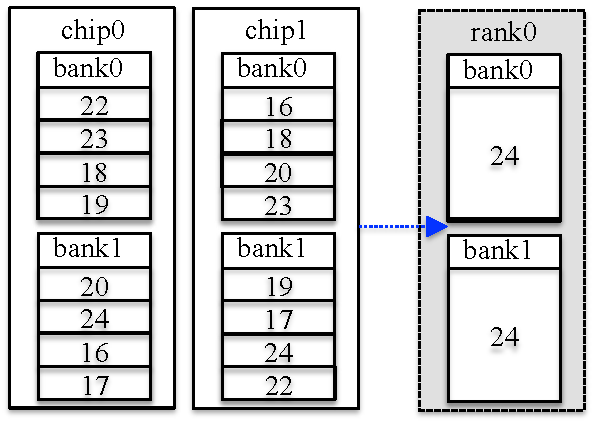
\includegraphics[width=\linewidth]{figures/default.pdf}\\
    \caption{Chip-specific}
    \label{fig:chip_default}
  \end{subfigure}
%
  \begin{subfigure}{.32\textwidth}
    \centering
    	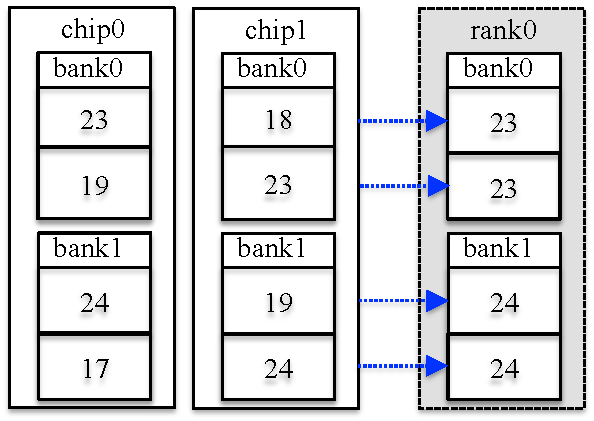
\includegraphics[width=\linewidth]{figures/chunk_unsort.pdf}\\
    \caption{Chunk-specific}
    \label{fig:chunk_unsort}
  \end{subfigure}
  %
  \begin{subfigure}{.32\textwidth}
    \centering
    	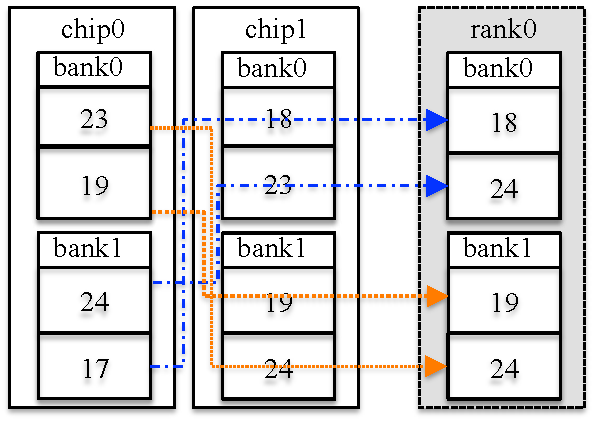
\includegraphics[width=\linewidth]{figures/chunk_sort.pdf}\\
    \caption{Chunk-specific w/ remap}
    \label{fig:chunk_sort}
  \end{subfigure}
  \vspace{-0.45in}
\caption{Comparison of different schemes: (a) The chip-specific {\tt tWR}; (b) The chunk-specific {\tt tWR}; (c) The chunk-specific {\tt tWR} with chunk remapping. For illustration purpose, each rank consists of two chips while each chip contains two four-row banks. One {\underline {\bf DIMM-row}} (i.e., the row exposed to the OS) consists of two {\underline {\bf chip-row}} segments --- the number in each chip-row indicates its corresponding {\tt tWR}, i.e., the {\tt tWR} of the weakest cell.}
\label{fig:schemes}
  \vspace{-0.45in}
\end{figure}

\subsection{Chunk-specific Restoring Control}
Even though {\tt tWR} exhibits a wide range of variations when scaling in deep sub-micron regime, only a small number of cells need long recovery time.  Setting a DIMM's {\tt tWR} based on the chip-row that has the worst {\tt tWR} is still too pessimistic.
We therefore propose to partition each memory bank into a number of smaller chunks and set the chunk level {\tt tWR} based on the worst chip-row within the chunk. 
The chunk level {\tt tWR} is then exposed to the memory controller to aid cheduling.

In Figure \ref{fig:schemes}(b), one chunk consists of two rows. Since the first chunk has 23ns and 18ns {\tt tWR}s for its two chip-rows, its chunk {\tt tWR} is set to 23ns.
By take advantage of these fast chunks, a chunk-{\tt tWR}-aware memory controller can speed up memory accesses that fall into the fast chunks
\footnote{For discussion purpose, a {\em chip-chunk} is referred to as one chunk within one chip; a {\em DIMM-chunk} is referred to as the set of same-index chip-chunks from different chips of the DIMM. For example, the 2nd DIMM-chunk consists of the 2nd chip-chunk from each chip.}.


\subsection{Chunk-specific with Remapping}

The previous design can only form a DIMM-chunk from the same-index chip-chunks, which can be optimized to further reduce {\tt tWR} values. This is because the chip-chunks that are of the same index may exhibit significant {\tt tWR} difference. It would be beneficial to form a chunk using chip-chunks that are of the same or similar {\tt tWR}s. 

For the example in Figure \ref{fig:chunk_sort}, if we form the first DIMM-chunk using the 4th chip-chunk from chip 0 and the 1st chip-chunk from chip 1, the {\tt tWR} of this chunk can be as low as 18ns. Constructing a number of such fast chunks helps to speed up the average row access time of the given DIMM.

The chunk remapping is done in two steps: (1) after detecting the {\tt tWR} for each chip-chunk, we compute the averaged {\tt tWR} for each chip-bank, and sort chip-banks independently on each chip. A {\bf DIMM-bank} consists of chip-banks that are of the same index on the sorted list; (2) For chip-chunks within each chip-bank, we sort them again such that each {\bf DIMM-chunk} consists of chip-chunks that are of the same index on the sorted list. 

While only one access is allowed to access one bank at any time, the multiple banks in a DIMM can be accessed simultaneously. To maintain the same bank level parallelism, we treat the chip-chunks from one bank as a group in chunk remapping. In Figure \ref{fig:schemes}(c), 
DIMM-chunk 0 and 1 belong the DIMM-bank 0. Since DIMM-chunk 0 is constructed using chip-chunk 3 on chip 0, DIMM-chunk 1 needs to use chunks from the same group, i.e., chip-chunk 2 on chip 0. In this way, simultaneously accessing two different DIMM-banks will never compete for the same chip-bank on any chip. 

\subsection{Restore Time aware Rank Construction}
\label{sec:match_twr}

A DIMM rank is composed of multiple chips, which work in lockstep fashion. The access speed of one logical row is determined by its worst chip-row. While chunk-remapping does not have to form a DIMM-row using the chip rows that of the same physical index, it may still be ineffective when one of the chips that form a rank contains many slow rows. A bad chip would lead to a slow rank no matter how the chunks are remapped.

\begin{figure}[ht]
\centering
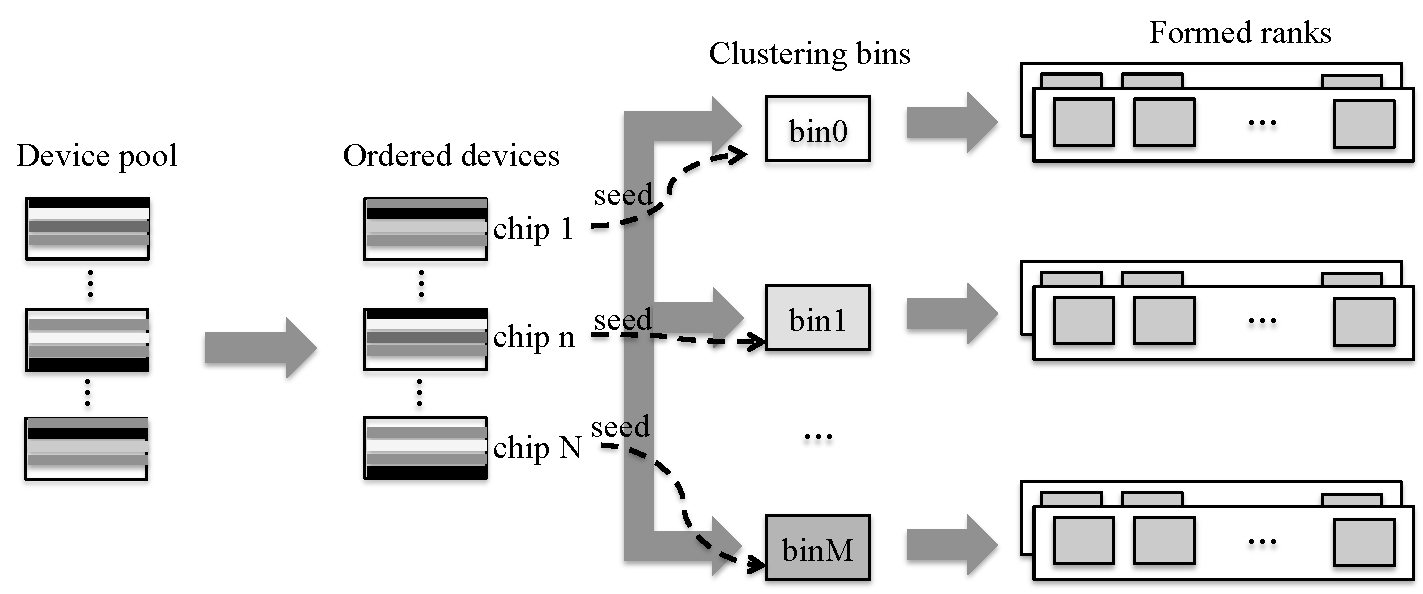
\includegraphics[width=0.8\textwidth]{figures/device_match.pdf}
\vspace{-0.15in}
\caption{Rank construction consists of three steps --- (1) chip sorting and seed chip selection;
(2) distributing chips to bins; (3) constructing DRAM ranks using chips from each bin.}
\label{fig:device_match}
  \vspace{-0.25in}
\end{figure}

We further propose to construct DRAM ranks using compatible chips, rather than random chip selection in the baseline design. 
Given $N$ DRAM chips, our goal is to construct a better rank set (and each rank contains $R$ chips). The rows in each chip are divided into $K$ chunks and we use $M$ bins to assist rank construction.

We first compute the average chip level {\tt tWR}, which uses the chunk level {\tt tWR} values of each chip. The latter can be collected during post-fabrication testing.
We sort the chips based on their average {\tt tWR} values, and choose $M$ seed chips, i.e., the chips on the sorted chip list whose indice can be divided by $\lfloor N/M\rfloor$. The seed chips are distributed to $M$ bins.

We then place the rest of chips into $M$ bins based on their similarity to the seed chip of each bin. The chunk level {\tt tWR} values of each chip are treated as a $K$-item vector. The similarity of two chips is calculated using the Hamming distance of the two $K$-item vectors. The candidate chip is placed in the bin whose seed chip has the smallest Hamming distance, i.e., the highest similarity, to the candidate chip.

Once a bin reaches its size limit, i.e., $n\times R$  where $n = \lfloor{N/M/R}\rfloor$, and $n\times R \leq N/M$, it can no longer accept new chips. In the algorithm, an extra bin $Bin_{M+1}$ is used to hold the leftover chips.
When filling chips to each bin, we construct a rank if a bin has $R$ chips (the seed chip is used to form a rank in the last batch). 

Since the algorithm needs to scan each chip and compute its similarity with all seed chips, the time complexity is $O(N\times M \times K)$. Here $M$ and $K$ are constant. $M$ is usually small ($M << N$) while $K$ can be relatively large, e.g., $K$=1024. Therefore, the time complexity is linear to the number of candidate chips. This is a light weight rank construction scheme, compared that in \cite{DAC15:radar}. Our experiments show that the two algorithms achieve similar rank level {\tt tWR} results. 
%. As a comparison, 
%the recently proposed rank construction scheme \cite{DAC15:radar} needs to sort the candidate chips continuously, which results in time complexity up to $O(N^3)$. 

\subsection{Restore Time aware Page Allocation}
\label{subsec:page_alloc}
%The translation of virtual to physical address is supported in hardware by Memory Management Unit (MMU), and the virtual-physical mapping is determined by operating system (OS). 
Traditional page allocation is restore time oblivious as all physical pages have the same access latency. However, when a set of fast DRAM chunks are constructed and exposed to the memory controller, %it is beneficial to exploit the access latency difference to speed up program execution. 
the memory system can be more effective if fast chunks are assigned to service performance-critical pages. In this paper, the page criticality is estimated using its access frequency \cite{ISCA13:charm,TC01:alloc}. Studies have shown that it is usually a small subset of pages, referred to as hot pages, that are frequently accessed in modern applications \cite{ISCA09:hot_page,ICS11:hot_page,TODAES13:hot_page}. %We adopt the offline profiling approach as in \cite{ISCA13:charm} to identify hot pages.

%\begin{figure}
 %\centering
 %   	\includegraphics[width=0.8\linewidth]{figures/TODAES_data/{page.dat}.pdf}\\
  %\vspace{-0.45in}
  %\caption{The page access distributions in SPEC CPU2006.}
  %\label{fig:page}
  %\vspace{-0.1in}
%\end{figure}


%Figure \ref{fig:page} studies the page access distribution of a set of SPEC CPU2006 applications. The figure shows that different applications have very different access behaviors: for some workloads, e.g., $459.Gem$ and $470.lbm$, accesses are evenly distributed such that the number of accumulative requests grows linearly with the number of touched pages; for some other applications, e.g., $429.mcf$ and $403.gcc$, most memory accesses come from a small subset of hot pages. The hot pages are the ones to be allocated in fast DRAM chunks. Further experimental analysis shows that the majority workloads touch less than 1/8 of the total memory space, while some benchmarks (i.e., $459.lbm$ and $429.mcf$) use up all available space.

In this paper, our goal is to illustrate that a restore time aware page allocator can take advantage of the latency difference of the DRAM chunks. For this purpose, we adopt a simple strategy that profiles program execution offline \cite{ISCA13:charm} and statically allocates hot pages to fast chunks. 
In the case if profiles are not accurate, we may need to design and enable more flexible strategies, e.g., such as the detailed behavioral synthesis \cite{TODAES11:partition} 
and data migration and compression \cite{TODAES08:bankmem}. We leave this as our future work. 

\section{Architectural Enhancements}
%In this section, we'll present the architectural implementations and also the overheads.

%\subsection{Implementation}
In order to exploit restore time variations at either chip or chunk levels, a post-fabrication testing needs to be performed to detect restore time at fine-granularity. Given that cell restore time is thermal dependent --- study showed that it becomes worse at low temperature \cite{MEM14:twr}, the manufacturer needs to record the worse timing constraints under chip's allowed working conditions. The values are organized as a table (with each entry in the table recording affected timing constraints {\tt tWR}/{\tt tRAS} of its corresponding DIMM chunk) and saved in non-volatile storage in the DIMM \cite{MICRO13:rowclone}. The memory controller loads this table at boot time and schedules memory accesses accordingly.% to maximize bandwidth and avoid conflicts. 
%As an example, two READ operations cannot be scheduled back to back to a DIMM bank if the later one accesses a fast chunk and shall compete with the preceding READ for using the data bus. 

\begin{figure}[ht] % !=overrides latex; h=here; t=top; b=bottom; p=special page for floating objects
\begin{center}
%\vspace{-0.1in}
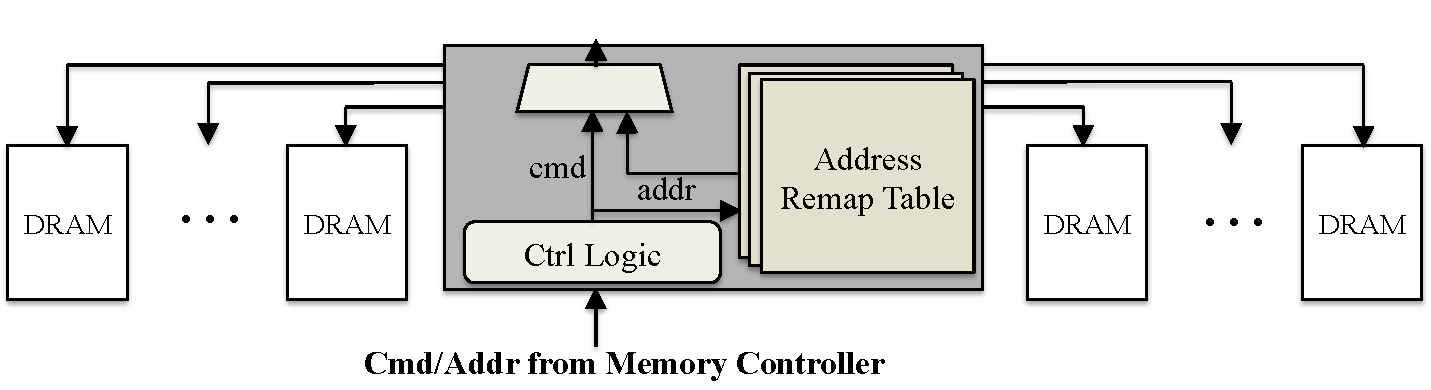
\includegraphics[width=0.7\textwidth]{figures/TODAES_data/design.pdf}
\vspace{-0.2in}
\caption{The on-DIMM architectural enhancement.}
\label{fig:design}
\end{center}
\vspace{-0.45in}
\end{figure}

To enable chunk re-organization, we need one extra chunk remapping table as shown in Figure \ref{fig:design}. Similar as HP's MC-DIMM \cite{SC09:mcdimm} and Mini-rank \cite{MICRO08:minirank}, our design integrates a bridge chip on-DIMM, which remaps the physical address sent from the memory controller to device row addresses in each chip. For the chunk remapping table, each entry maps the corresponding DIMM-chunk to the chip-chunk at each chip.  
%Given the following Table \ref{tab:art}, when the bridge chip receives a request asking for data in the 10th DIMM-chunk, it translates the requests to asking for segment data from the 1220$^{th}$ chunk from chip 0, the 124$^{th}$ chunk from chip 1, etc. 

%\begin{table}[htbp]
%\centering
%\caption{Remap table}
%\begin{tabular}{cccccccc}
%\hline
%DIMM\_chunk &chip0\_chunk &chip1\_chunk &... &chip7\_chunk \\
%\hline 
%...	 	&...	&... 	&...		&...\\
%10	 	&1220		&124 	&...		&256\\
%...	 	&...	&... 	&...		&...\\
%\hline 
%\end{tabular}
%\vspace{-0.2in}
%\label{tab:art}
%\end{table}

\section{Experimental Methodology}
\subsection{Configuration}
To evaluate the effectiveness of our designs, we compared them to traditional repair solutions using an in-house chip-multiprocessor system simulator. We modeled a quad-core system with the parameters shown in Table \ref{tab:configuration}. 

We used VARIUS to generate 90 chips, and then form ranks in different fashion discussed in Section \ref{sec:match_twr}. The memory system to be simulated is composed of two ranks. We constructed five rank pairs and tested the proposed designs with all pairs.
The DRAM timing constraints follow Hynix DDR3 SDRAM data sheet \cite{hynix:ddr3}. 
%For the schemes exploiting chunk level timing constraints, we added two CPU cycles to access the timing table.
%For the schemes performing chunk-remapping, we added one extra DRAM cycle to access the mapping table.

\begin{table}[htbp]
\vspace{-0.2in}
\centering
\caption{System Configuration}
\vspace{-0.15in}
\scalebox{0.85}
{
\begin{tabular}{l|l}
\hline\hline
Processor				&four 3.2Ghz cores; four-issue; 128 ROB size\\
\hline
				&L1(private): 64KB, 4-way, 3 cycles\\
Cache			&L2(shared): 2MB, 6-way, 32 cycles\\
				&64B cacheline\\
\hline
Memory				&Bus frequency: 1066 MHz\\
Controller 	& 128-entry queue; close page\\
\hline
			&1channel, 2ranks/channel, 8banks/rank, \\
DRAM				&16K rows/bank, 8KB/row,\\
				&1066 MHz, tCK=0.935ns, width: x8\\
\hline\hline

\end{tabular}
}
\label{tab:configuration}
\vspace{-0.2in}
\end{table}

\subsection{Workloads}
We used SPEC CPU2006 and simulated 1 billion instructions after skipping the warm-up phase of each benchmark. 
%The Read and Write MPKI (memory accesses per kilo instructions) for each workload is profiled to indicate the memory intensiveness. 
Based on MPKI, the applications are classified into three categories (Spec-High/Spec-Med/Spec-Low).%, as shown in Table \ref{tab:bench}.
The workloads are running in rate mode, where all cores execute the same task.

We performed timing simulation until all cores finish the execution, and averaged the execution time of all the four cores. We constructed five rank pairs, i.e., DIMMs. One simulation run used one DIMM while the reported results are the average of the runs using different DIMMs.

\section{Results}
We evaluated the following schemes:

--- \texttt{Baseline}. The baseline sets {\tt tWR} to 15ns, following existing specification. It is the ideal baseline due to scaling. The results of other schemes are normalized to the baseline for comparison.

--- \texttt{Relax-}$x$. Given that scaling in deep sub-micron regime leads to worse timing, this scheme relaxes time constraints to achieve x\% yield. We relaxed {\tt tWR} and set {\tt tRAS}/{\tt tRC} accordingly. We tested x=85 and x=100, respectively.

--- \texttt{Spare-}$x$. One commonly adopted post-fabrication repair approach is to integrate sparing rows/columns \cite{BOOK:jacob} to mitigate performance and yield loss. 
%It is implemented by using a laser programmable link to disconnect the abnormal rows/columns and connect the spare ones \cite{Bruce:Jacob}. 
In our experiments, we set the spare density as high as 16 spare rows per 512-row block, which resides in the aggressive spectrum \cite{BOOK:fault,SSC96:spare}. Given that spares may be reserved for high-priority repairs, such as defects and retention failures, we testsed x=0, 2, 8, 16 spares out of each 512-row block, respectively. 

--- \texttt{ECC}. ECC is implemented by placing one extra ECC chip to correct errors in data chips. Though ECC is conventionally used to correct soft errors, it can be potentially used to tolerate weak cells. Exploiting ECC chips to rescue slow rows sacrifices soft error resilience and hurts reliability \cite{DFT05:ecc}.  

--- {\tt Chunk-}$x$. This scheme implements the chunk-specific restore time control, with each bank being divided into $x$ chunks. Each DIMM chunk has its own timing constraints, which are exposed to the variation-aware memory controller.

--- \texttt{ChunkSort-}$x$. This scheme implements the chunk-specific restore time control with chunk remapping, with each bank being divided into $x$ chunks. Similar as {\tt Chunk-}$x$, the timing constraints of each chunk are exposed to the memory controller.

--- \texttt{ChunkBin-}$x$. This schemes is similar as {\tt Chunk-}$x$. The difference is that it constructs ranks using the proposed bin-based matching scheme.

--- \texttt{ChunkSortBin-}$x$.  This schemes is similar as {\tt ChunkSort-}$x$. The difference is that it constructs ranks using the proposed bin-based matching scheme.

We compared these schemes on memory access latency and system performance, and studied their sensitivity to different system configurations. 

\subsection{Execution Time}

\begin{figure}[ht]
\centering
\includegraphics[width=0.7\textwidth]{figures/TODAES_data/14nm/{stat_RAND_main-cycles.perc.dat}.pdf}
\vspace{-0.2in}
\caption{The execution time comparison of different schemes under random page allocation policy. Representative applications and the geometric means for highly memory-intensive (Spec-High) and all applications (Spec-All) are presented here.}
\label{fig:tech_time}
  \vspace{-0.25in}
\end{figure}

From Figure \ref{fig:tech_time}, we observed that 
(1) DRAM scaling has a large impact on restore time. To maintain a high yield rate, the timing constraints have to be vastly relaxed from 16 cycles to over 40 cycles, which significantly hurts performance. On average, {\tt Relax-100} and {\tt Relax-85} prolong the execution time by 37.0\% and 34.9\%, respectively. Highly memory-intensive applications tend to have large degradation (i.e., over 40\%). 
(2) Adding spare rows helps to mitigate performance losses: {\tt Spare-8} is 31.9\% worse than the ideal. 
(3) {\tt ECC} works only slightly better than {\tt Spare-8}. This is because SEC-DED ECC can only correct one bit in each 64-bit block. Since there  might be multiple cells violating timing constraints within such a 64-bit block, ECC lacks the ability to effectively adapt restore time variations.
(4) {\tt Chunk-4k} is less than 1\% better than {\tt ECC} as it exposes chunk-level restore time variations. There are a small number of chunks that have smaller tWRs than the single tWR in {\tt ECC}. Due to random page allocation policy, the exposed fast chunks cannot be fully exploited, and thus the performance improvement is pretty limited.
(5) {\tt ChunkSort-4k} works better than {\tt Chunk-4k} because it helps to construct more fast chunks. On average,
{\tt ChunkSort-4k} helps to reduce the performance loss from 37\% in {\tt Relax-100} to 26.5\%, and 4\% better than {\tt Chunk-4k} for {\tt Spec-High}.

In addition, restore time aware rank construction helps to reduce tWR ---  {\tt ChunkBin-4k} is 3\% better than  {\tt Chunk-4k} while  {\tt ChunkSortBin-4k} is 4.8\% better than  {\tt ChunkSort-4k}. 
Interestingly, {\tt ChunkBin-4k} and {\tt ChunkSort-4k} achieve comparable performance improvements over the baseline. While both schemes require post-chip-fabrication testing to extract chunk level tWR values, the former needs rank clustering, which imposes extra step and cost during fabrication; the latter needs to embed mapping table and thus introduces extra runtime overhead.  
{\tt ChunkSortBin-4k} achieves the best performance while it incurs both extra fabrication cost and runtime overhead. 

\subsection{Page Allocation Effects}

Figure \ref{fig:tech_time_14nm} compare the results using random and restore-time-aware page allocation schemes.
From the figure, by making better use of fast chunks, restore time aware page allocation speeds up the execution of all chunk based schemes, e.g., for {\tt ChunkSortBin-4k}, restore time aware allocation achieves 15\% improvement over random allocation.
Restore time aware allocation is very effective for most benchmark programs --- on average, {\tt ChunkSortBin-4k} is only 2\% worse than the ideal {\tt Baseline}. 

\begin{figure}
\centering

\begin{minipage}[b]{0.42\linewidth}
\centering
\includegraphics[width=\linewidth]{figures/TODAES_data/14nm/{RAND_small.dat}.pdf}\\
\subcaption{With random page allocation}%\label{fig:20nm_main}
\end{minipage}%
\begin{minipage}[b]{0.42\linewidth}
\centering
\includegraphics[width=\linewidth]{figures/TODAES_data/14nm/{PROF_small.dat}.pdf}\\
\subcaption{With restore time aware page allocation}%\label{fig:14nm_main}
\end{minipage}%
\vspace{-0.4in}
\caption{The execution time comparison of different schemes at 14nm technology node.}
\label{fig:tech_time_14nm}
\vspace{-0.45in}
\end{figure}


In the figure, $470.lbm$ achieves small improvement because it evenly accesses a large number of memory pages and lacks very hot pages.  Given that a small number of chunks have shorter than 15ns tWR values, it is not surprising to find that some benchmark programs, e.g., $403.gcc$ and $400.per$, have their hot pages fit in these fast chunks and thus outperform {\tt Baseline}.

Also in the figure, we observed that the effectiveness of restore time aware rank construction is diminishing after adopting restore time aware allocation. For example, on average, {\tt ChunkSort-4k} and {\tt ChunkSortBin-4k} have less than 1\% difference when using restore time aware allocation. 
Nevertheless, those benchmarks with large footprint and relatively uniform access pattern, e.g., $470.lbm$, can still achieve distinct benefits.

\subsection{Further Studies}
The effectiveness of conventional Sparing technique strongly depends on the sparing levels being used; the proposed chunk-based schemes depends on the chunk granularity. Hence, we conducted sensitivity studies on these two key parameters. 
And the experimental results show that diminishing returns using more spares because of increasingly more slow cells.
As expected, the study varying number of chunks shows that higher improvement can be achieved with increasing storage and latency overheads.

\section{Conclusion}
In this work, we studied DRAM scaling effects on restore time, and showed that future DRAM chips need relaxed timing constraints to maintain high yield and to keep the manufacturing cost low. Existing approaches are ineffective to address the performance losses. 
We proposed schemes to expose restore time variations at chunk level and devised architectural enhancements to enable find-grained variation-aware scheduling. We then proposed restore time aware rank construction and page aware page allocation schemes to make better use of fast chunks. The experimental results show that our schemes achieve as high as 25\% average performance improvement over traditional solutions.



\chapter{Shorten Restoring using Refresh}
\label{chapter:partialrestore}
%\section{Background on Refresh}
%DRAM needs to be refreshed periodically to prevent data loss. According to JEDEC \cite{JEDEC:ddr3}, 8192 all-bank auto-refresh ({\tt REF}) commands are sent to all DRAM devices in a rank within one retention time interval ({\tt Tret}), also called as one refresh window ({\tt tREFW}) \cite{TC15:refresh, ISCA13:ddr4, HPCA14:parallelrefresh}, typically 64ms for DDR3/4. The gap between two {\tt REF} commands is termed as refresh interval ({\tt tREFI}), whose typical value is 7.8$\mu$s, i.e. 64ms/8192.If a DRAM device has more than 8192 rows, rows are grouped into 8192 {\bf refresh bins}. One {\tt REF} command is used to refresh multiple rows in a bin. An internal counter in each DRAM device tracks the designated rows to be refreshed upon receiving {\tt REF}. The refresh operation takes {\tt tRFC} to complete, which proportionally depends on the number of rows in the bin.

%The refresh rate of one bin is determined by the leakiest cell in the bin. Liu~{\em et~al.} \cite{ISCA12:raidr} reported that fewer than 1000 cells require a refresh window shorter than 256ms in a 32GB DRAM main memory. Given that the majority of rows have retention time longer than 64ms, it is beneficial to enable multi-rate refresh, i.e., different bins are refreshed at different rates. The weakest cell in one bin determines the refresh rate of the bin. For discussion purpose, a DRAM cell/row/bin that is refreshed at 256ms is referred to as a \underline{256ms-cell}/\underline{row}/\underline{bin}, respectively.

%We adopt the {\em flexible auto-refresh} mechanism from \cite{ISCA15:reflex} to support multi-rate refresh, i.e., 8192 refresh commands are sent every 64ms --- one for each bin. If a bin needs to be refreshed every 256ms,  {\em flexible auto-refresh} sends four {\tt REF} commands in 256ms to this bin. However, only one is a real refresh while the other three are dummy ones that only increment the refresh counter. 

%While the bin counter is maintained in the memory controller and incremented sequentially, the actual row addresses (responding to each bin-refresh command) are generated internally inside DDR3/4 devices \cite{JEDEC:ddr3,JEDEC:ddr4}. This mapping may be non-linear because of vendor's full flexibility to implement the refresh.Recent studies \cite{ISCA15:reflex, ISCA14:disturbance} assume this mapping can be made known to the memory controller. We make the same assumption in this paper.
%We assume that the memory controller knows the mapping between bin address and row address, the same as that in \cite{ISCA15:reflex}, and similar to \cite{ISCA14:disturbance}.

\section{Motivation of Partial Restore}
Due to intrinsic leakage, the voltage level of a DRAM cell reduces monotonically after a full restore. The solid curve in Figure \ref{fig:partial} illustrates the voltage decay of an untouched cell (i.e., not accessed) within one refresh window, commonly 64ms. Stored data is safe as long as the voltage remains above V$_{min}$ (0.73V$_{dd}$
\footnote{Value is calculated on basis of charge sharing expression \cite{BOOK13:sharing} and offset noise \cite{JSSC02:sense}, details can be found in \cite{HPCA16:twr}.}
 here)  before the next refresh. If a read or write access occurs, the post-access restore operation fully charges the cell, as shown in the figure. However, the full charge is often unnecessary if the access is {\em close in time} to the next refresh, which will fully restore the cell anyway.

\begin{figure}[htbp]
\begin{center}
%\vspace{-0.2in}
\centering
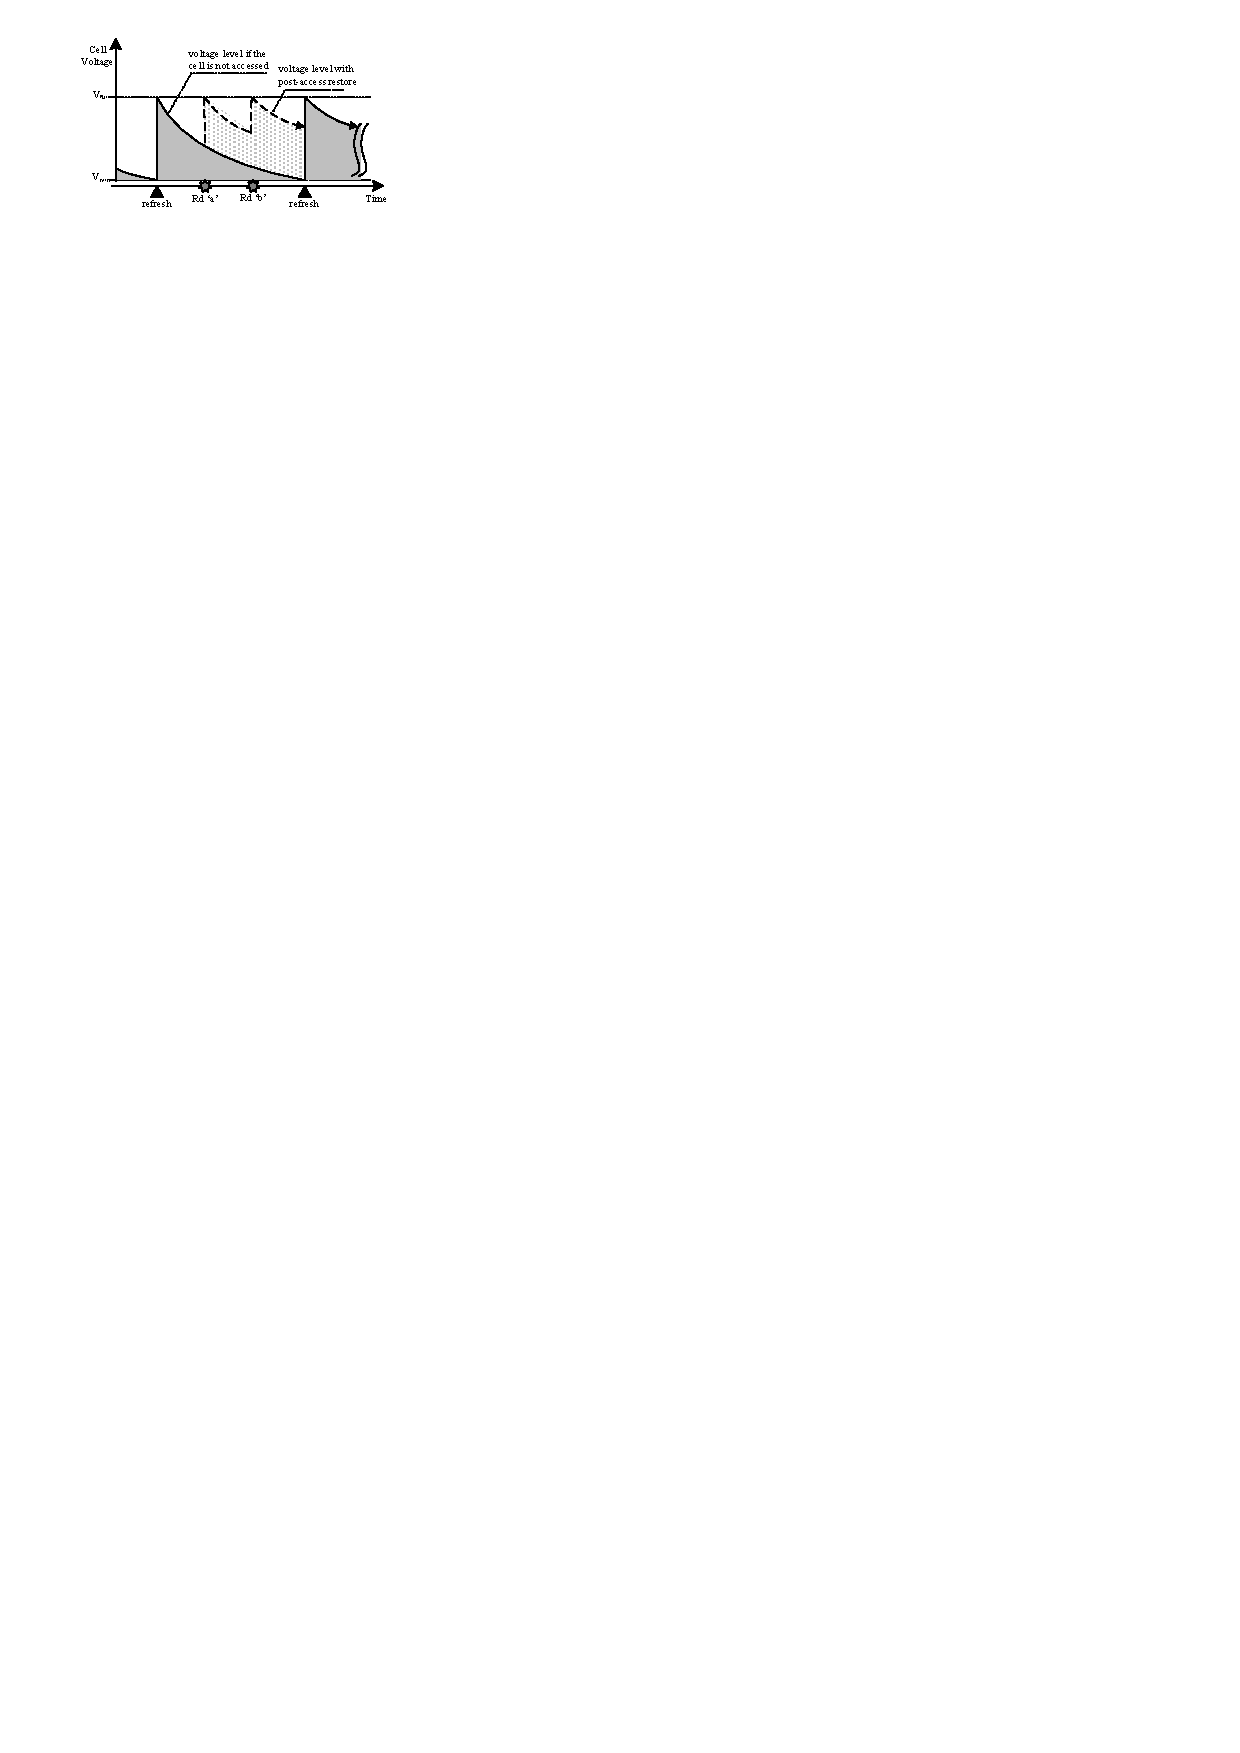
\includegraphics[width=3.2in]{figures/HPCA16/rt_partial.pdf}
\vspace{-0.2in}
\caption{DRAM cell voltage is fully restored by either refresh commands or memory accesses.  (V$_{full}$ indicates fully charged; V$_{min}$ is the minimal voltage to avoid data loss).}
\label{fig:partial}
\vspace{-0.3in}
\end{center}
\end{figure}

Based on this observation, we propose that post-access restore {\em partially charges} a cell's voltage to the level that the cell would have if the cell had been untouched in one refresh window. The restore operation is terminated when this target voltage level is reached. 

The cell charging curve starts with a deep slope and flattens when approaching V$_{full}$ \cite{HPCA15:aldram, PATENT11:dram}, as demonstrated in SPICE modeling. Hence, reducing target voltage can drastically shorten restore time. For example, SPICE modeling indicates that restoring a cell's charge to 0.89 V$_{dd}$ rather than 0.975 V$_{dd}$ (fully charged) reduces {\tt tWR} from 25 to 15 DRAM cycles, i.e., a 40\% reduction.

We next describe two schemes, {\tt RT-next} and {\tt RT-select}, to enable partial restore.  These schemes are applied by the memory controller.

\section{Proposed Designs}
\subsection{RT-next: Refresh-aware Truncation}

\begin{savenotes}
\begin{table*}[htbp]
\vspace{-0.2in}
\begin{center}
\caption{Adjusted restore timing values in {\tt RT-next}  (using the SPICE model)}
\vspace{-0.15in}
\label{rt_next_timing}
\scalebox{0.75}
{
\begin{tabular}{|c||c|c|c|c|*3c|}
\hline\hline
sub-window& \multicolumn{3}{|c|}{Distance to next refresh} & Target restore     &{\tt tRAS}	  &{\tt tWR}	  &{\tt tRCD}\\
            & 64ms-row & 128ms-row & 256 ms-row              & voltage (V$_{dd}$) &\multicolumn{3}{c|}{(DRAM cycles) \footnote{Timing values are gotten from SPICE modeling, more details can be found in \cite{HPCA16:twr}.}} \\ \hline \hline
1st         & [64ms, 48ms) & [128ms, 96ms) & [256ms, 192ms)  & 0.975		&42		&25	   	&15 \footnote{The studies focus on the relationship between restore and retention. Consequently, unrelated timing values, such as {\tt tRCD}, are unchanged.}  \\ \hline
2nd         & [48ms, 32ms) & [96ms, 64ms) & [192ms, 128ms)   & 0.92          	&27      &18    	&15  \\ \hline
3rd         & [32ms, 16ms) & [64ms, 32ms) & [128ms, 64ms)    & 0.86          	&21      &14    	&15  \\ \hline
4th         & [16ms, 0ms) & [32ms, 0ms) & [64ms, 0ms)        & 0.80          	&18      &11     &15  \\ \hline \hline
\multicolumn{4}{|c|}{No Truncation}            &0.975		&42		&25    	&15  \\ \hline \hline
%refresh margin &0.73          	&15      &9     &15  \\ \hline \hline
\end{tabular}
}
\end{center}
\vspace{-0.1in}
\end{table*}
\end{savenotes}

{\tt RT-next} truncates a long restore operation according to the time distance to its next refresh. %The sooner the next refresh is, the less charge the cells in the row need, and the earlier the restore operation can be terminated.  
%{\tt RT-next} works as follows. 
The refresh window is partitioned into multiple sub-windows, each of which provides a set of timing parameter values.
In the following, we use four sub-windows to discuss our proposed schemes --- Table \ref{rt_next_timing} lists the adjusted timing values for the device that we model in this paper. The smaller the timing values are, the larger opportunity the truncation has. While distinguishing more sub-windows provides finer-grained control and the potential to exploit more truncation benefits, it complicates the control and has diminishing benefits as shown in our experiments. 

As illustrated by Figure~\ref{fig:rtnext}, when servicing a read or write access, {\tt RT-next}  
calculates the time distance to the next refresh command and determine the sub-window that the access falls in. It then truncates its restore operation using the adjusted timing parameters, e.g., the right most columns in Table \ref{rt_next_timing}.

\begin{figure}[htbp]
\begin{center}
%\vspace{-0.1in}
\centering
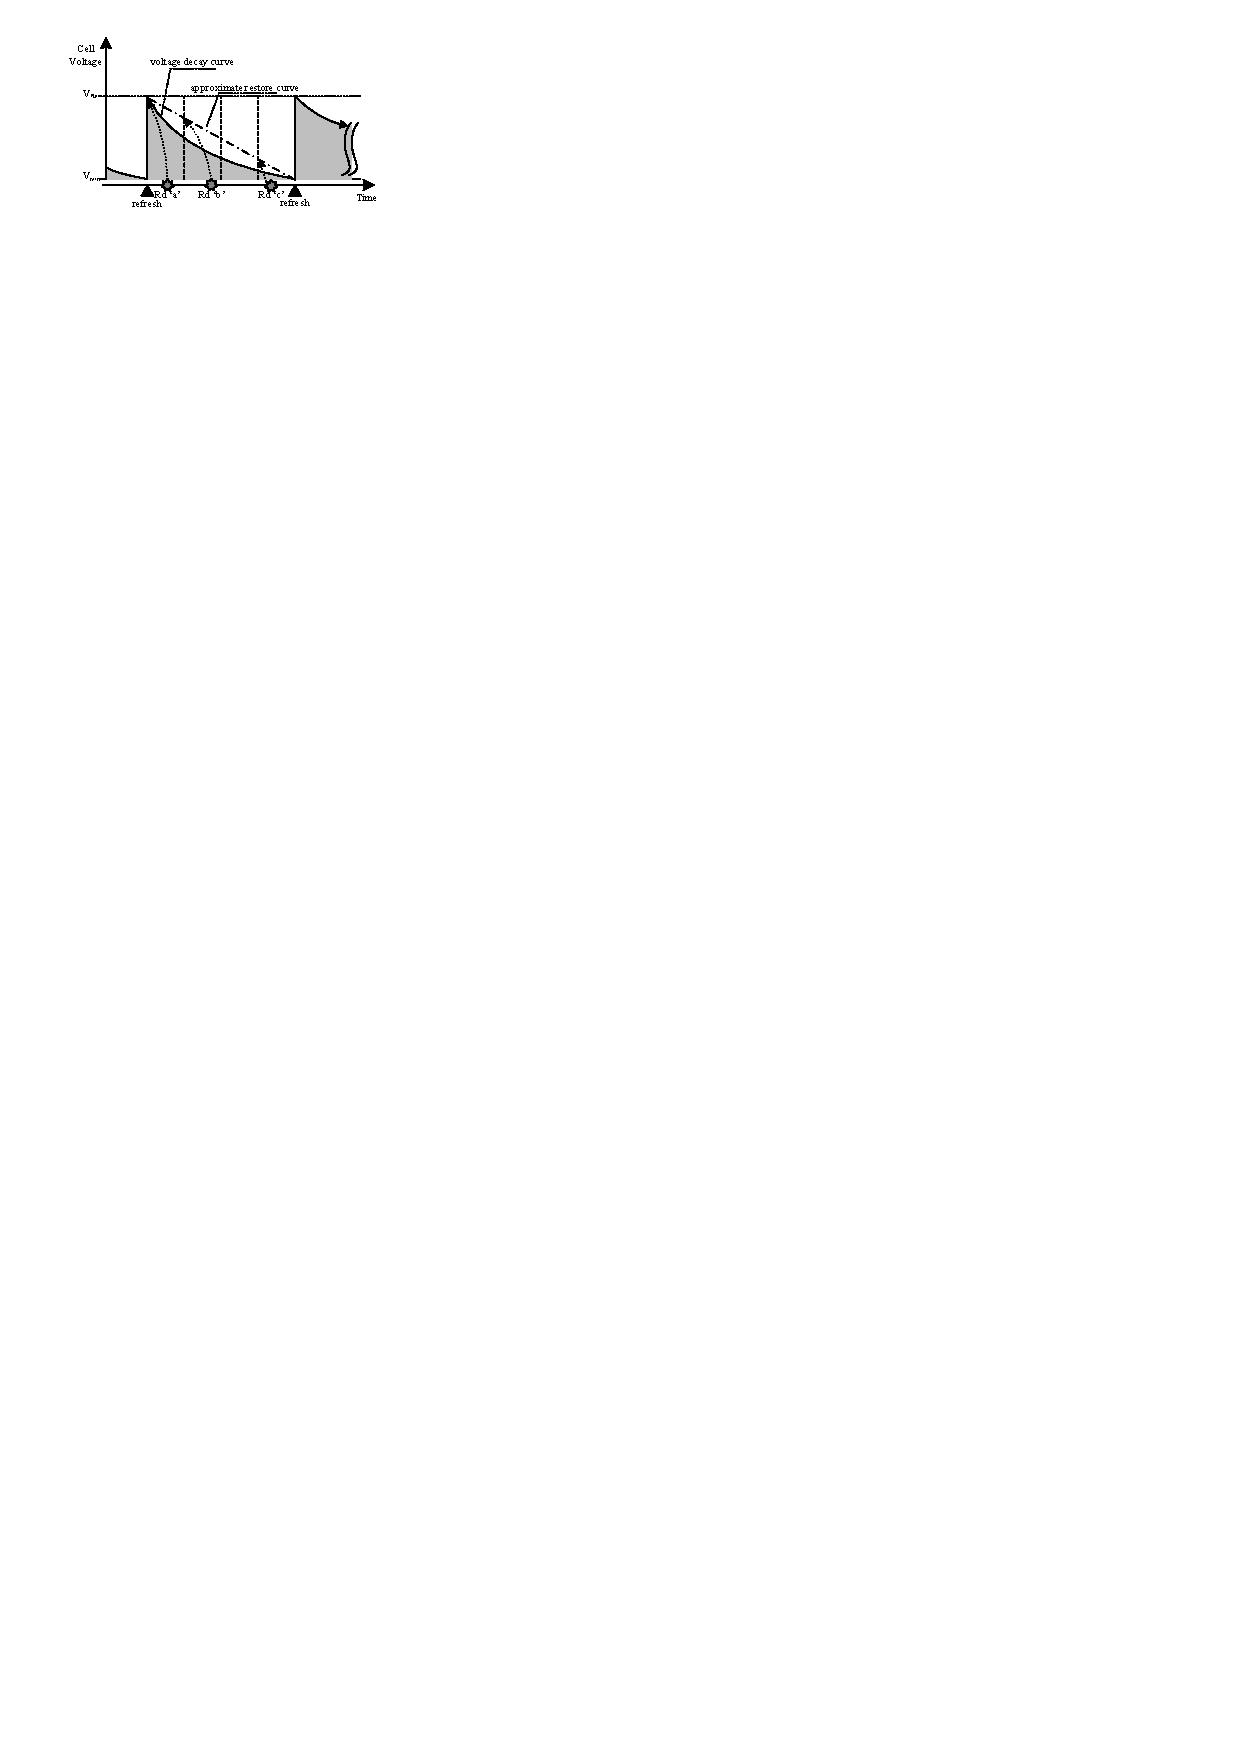
\includegraphics[width=3.2in]{figures/HPCA16/rt_next.pdf}
\vspace{-0.2in}
\caption{{\tt RT-next} safely truncates restore operation. Exponential curve has been verified from SPICE modeling, and linear line shows the conservative restoring goals.}
\label{fig:rtnext}
\vspace{-0.45in}
\end{center}
\end{figure}

%The memory controller also needs to consider the page policy (open or close).  A restore is truncated by a {\tt PRE} command from the memory controller. 
%For a close-page policy, every access can potentially truncate restore early. 
%For an open-page policy, truncating restore of a preceding access may not beneficial if its following access is a row buffer hit. 
%We evaluate both policies in the experiments.

%Figure~\ref{fig:rtnext} illustrates the working mechanism of {\tt RT-next}, where reads {\tt 'a'}, {\tt 'b'}, and {\tt 'c'} are serviced in the first, the second, and the fourth sub-windows, respectively.  Generally, {\tt RT-next} is a conservative approach to restore the cell charge.
%The figure shows how {\tt RT-next} is conservative in two ways:



%\footnotetext{\hi{Note that the negative slope is the conservatively approximated restore curve; the voltage decay curve, not shown in the figure, is always below the restore line.}}

%{\tt RT-next} is compatible with baseline auto refresh policy \cite{ISCA15:refresh, JEDEC:ddr3} that sends out {\tt REF} commands sequentially for all refresh bins. Given a DRAM row being accessed, the memory controller checks which bin the last {\tt REF} command is for and then determine how far the {\tt REF} is to be sent for the bin that the being accessed row resides.

\vspace{0.1in} 
{\underline{\bf {\tt RT-next} in multi-rate refresh.}}
\footnote{Retention time is modeled following \cite{EDL09:ret,ISCA12:raidr,ISCA13:archshield}, and leaky cells are randomly distributed based on prior works \cite{ISCA12:raidr, ISCA15:reflex, ICCD14:proactive}}
Applying {\tt RT-next} in a multi-rate refresh environment works similarly to the case that has only one rate. To calculate the distance between a memory access and the next refresh to its bin, 
{\tt RT-next} uses the same formula except adding the extra refresh rounds for low rate, i.e., 128/256ms, bins.
%replacing the refresh rate value with the individual refresh rate attached to each bin. 
Here we assume the underlying multi-rate refresh scheme has profiled and tagged each bin with its best refresh rate, e.g., 64ms, 128ms, or 256ms. 

As shown in Figure \ref{fig:rtnext_m}, it simplifies the timing control in memory controller by restoring a cell's post-access voltage according to the linear line between V$_{full}$ and V$_{min}$ (rather than the exponential decay curve). Given a 64ms-row and a 256ms-row, accesses falling in the same corresponding sub-window can use the same timing values in Table \ref{rt_next_timing}. 

\begin{figure}[htbp]
\begin{center}
\vspace{-0.1in}
\centering
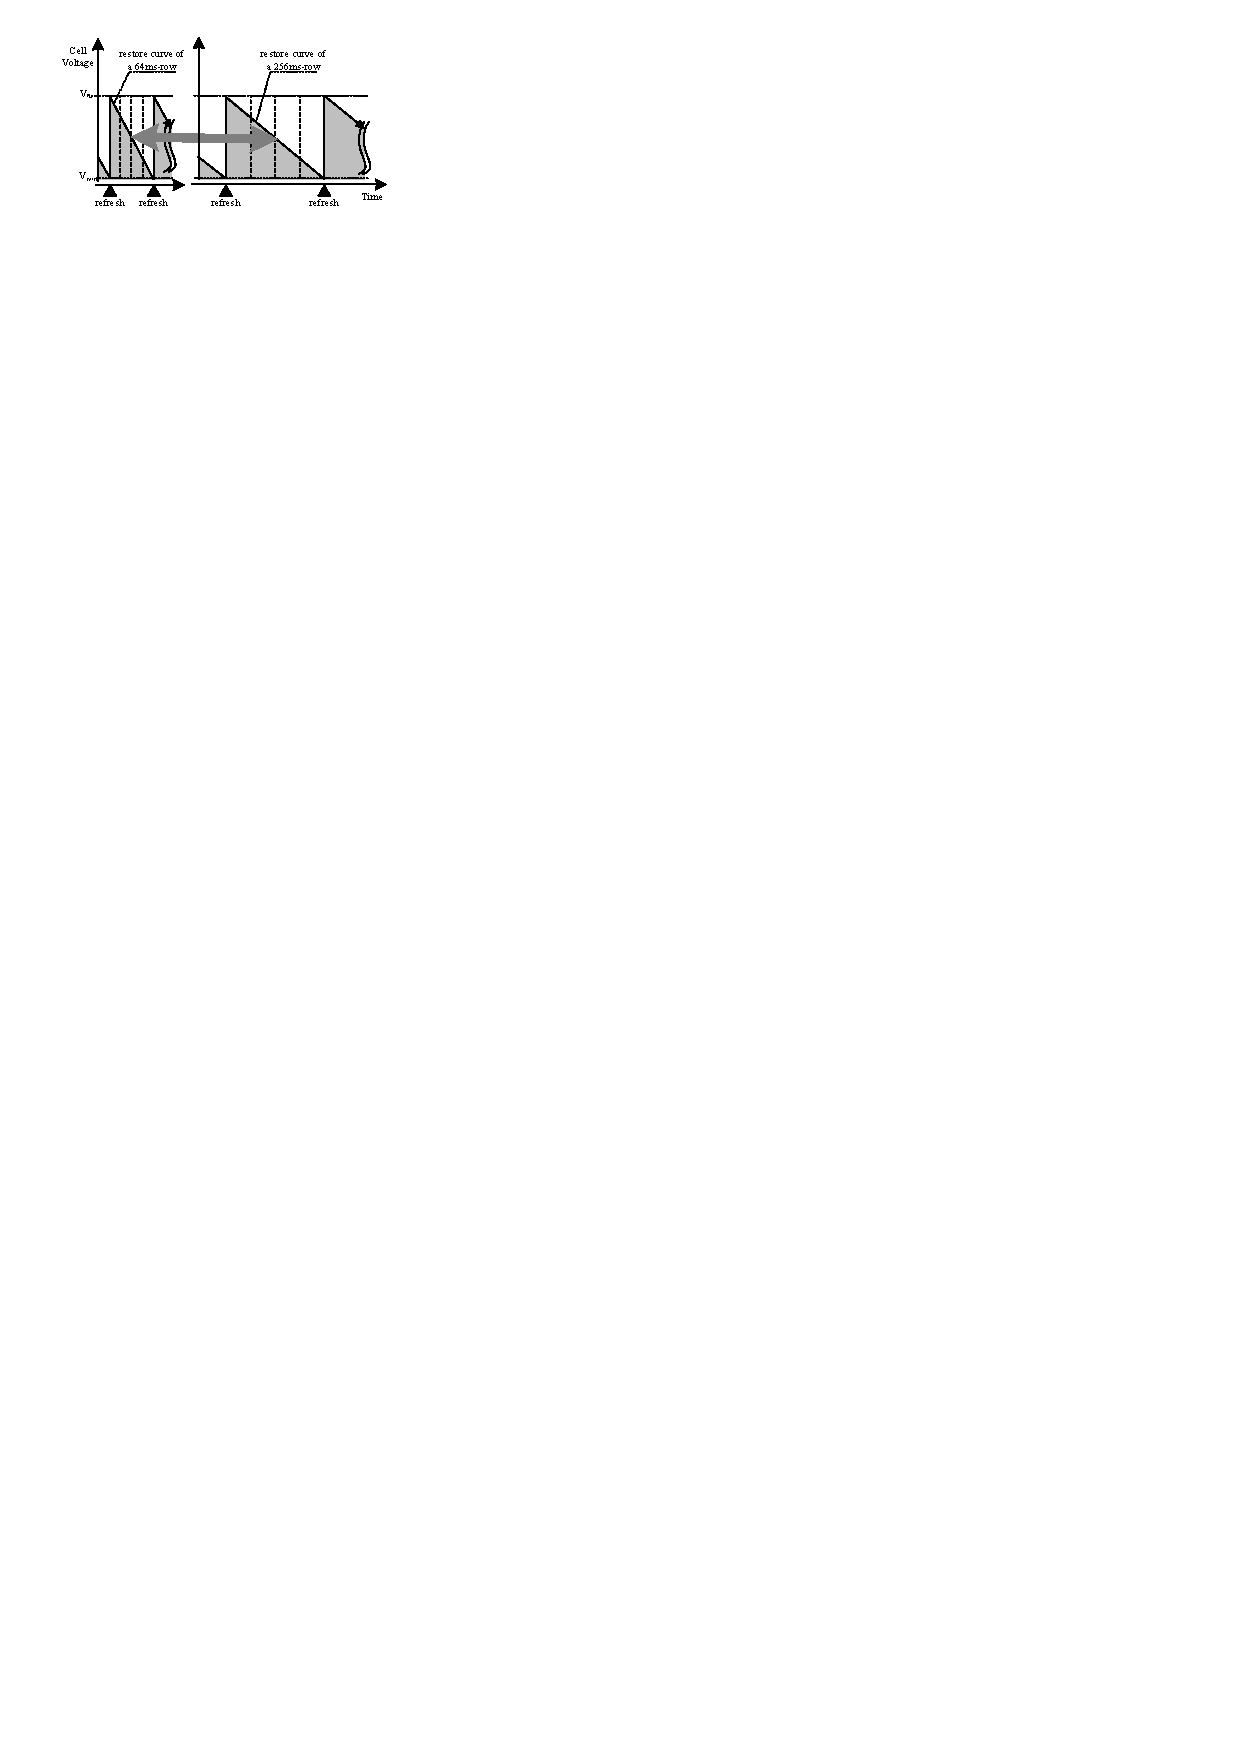
\includegraphics[width=3.2in]{figures/HPCA16/rt_next_m.pdf}
\vspace{-0.2in}
\caption{Restoring voltage according to linear line simplifies timing control in multi-rate refresh --- a 64ms-row and a 256ms-row share the same timing values in each correspond sub-window.}

\label{fig:rtnext_m}
\vspace{-0.45in}
\end{center}
\end{figure}

%In particular, although two different bins (e.g., 64ms and 256ms bins) have different sub-interval durations, they use the same adjusted timings (see Table \ref{rt_next_timing}). The same timings are used because, as shown in Figure \ref{fig:rtnext_m}, restore is conservatively performed using the approximated linear curve. 
%The cell loses about the same portion of charge within each sub-interval.
%The cell necessitates the same portion of charge within each sub-interval.
%\hi{Such interval division minimizes the required number of timing sets and thus greatly simply the design of memory controller}


\subsection{RT-select: Proactive Refresh Rate Upgrade}
Refresh and restore are two correlated operations that determine the charge in a cell. Less frequently refreshed bins can be exploited to further shorten the post-access restore time. 
We next present {\tt RT-select}, a scheme that upgrades refresh rate for more truncation opportunities. 

Figure \ref{fig:rtselective} illustrates the benefit of refreshing a 256ms-row (in multi-rate refresh) at 128ms rate.  Given that this row is a 256ms-row, its voltage level decreases to V$_{min}$ after 256ms. As shown in Figure \ref{fig:rtselective}(a), the refresh commands sent at +64ms, +128ms, and +192ms marks are dummy ones. The access ``Rd'' appears in the 2nd sub-window; it has a distance within [192ms, 128ms) to the next refresh command. According to {\tt RT-next}, the restore can be truncated after reaching 0.92V$_{dd}$ (using the 256ms-row column in Table \ref{rt_next_timing}).

Now, suppose the dummy refresh at +128ms is converted to a real refresh, i.e.,  the row is ``upgraded'' to a 128ms-row.  With this earlier refresh, 
%However, if the {\em dummy refresh at 128ms is converted to a real refresh (i.e., the 
%row is upgraded to a 128ms-row), then 
the access ''Rd'' is at most 64ms away from the next refresh. 
Using the 128ms-row column in the timing adjustment table, {\tt RT-next} 
can truncate the restore after it reaches 0.86V$_{dd}$, achieving significant timing 
reduction for the restore operation (Figure \ref{fig:rtselective}(b)).

%{\underline{if we convert the dummy refresh}}
%{\underline{command at 128ms mark to a real refresh, i.e., this row is}} \\
%{\underline{upgraded to a 128ms-row}}, access ``R$_a$'' is at most 64ms away from its next refresh. Using the 128ms-row column in the timing adjustment table, {\tt RT-next} can truncate the restore after it reaches 0.86V$_{dd}$, achieving significant timing reduction in restore operations.

\begin{figure*}[htbp]
\begin{center}
%\vspace{-0.1in}
\centering
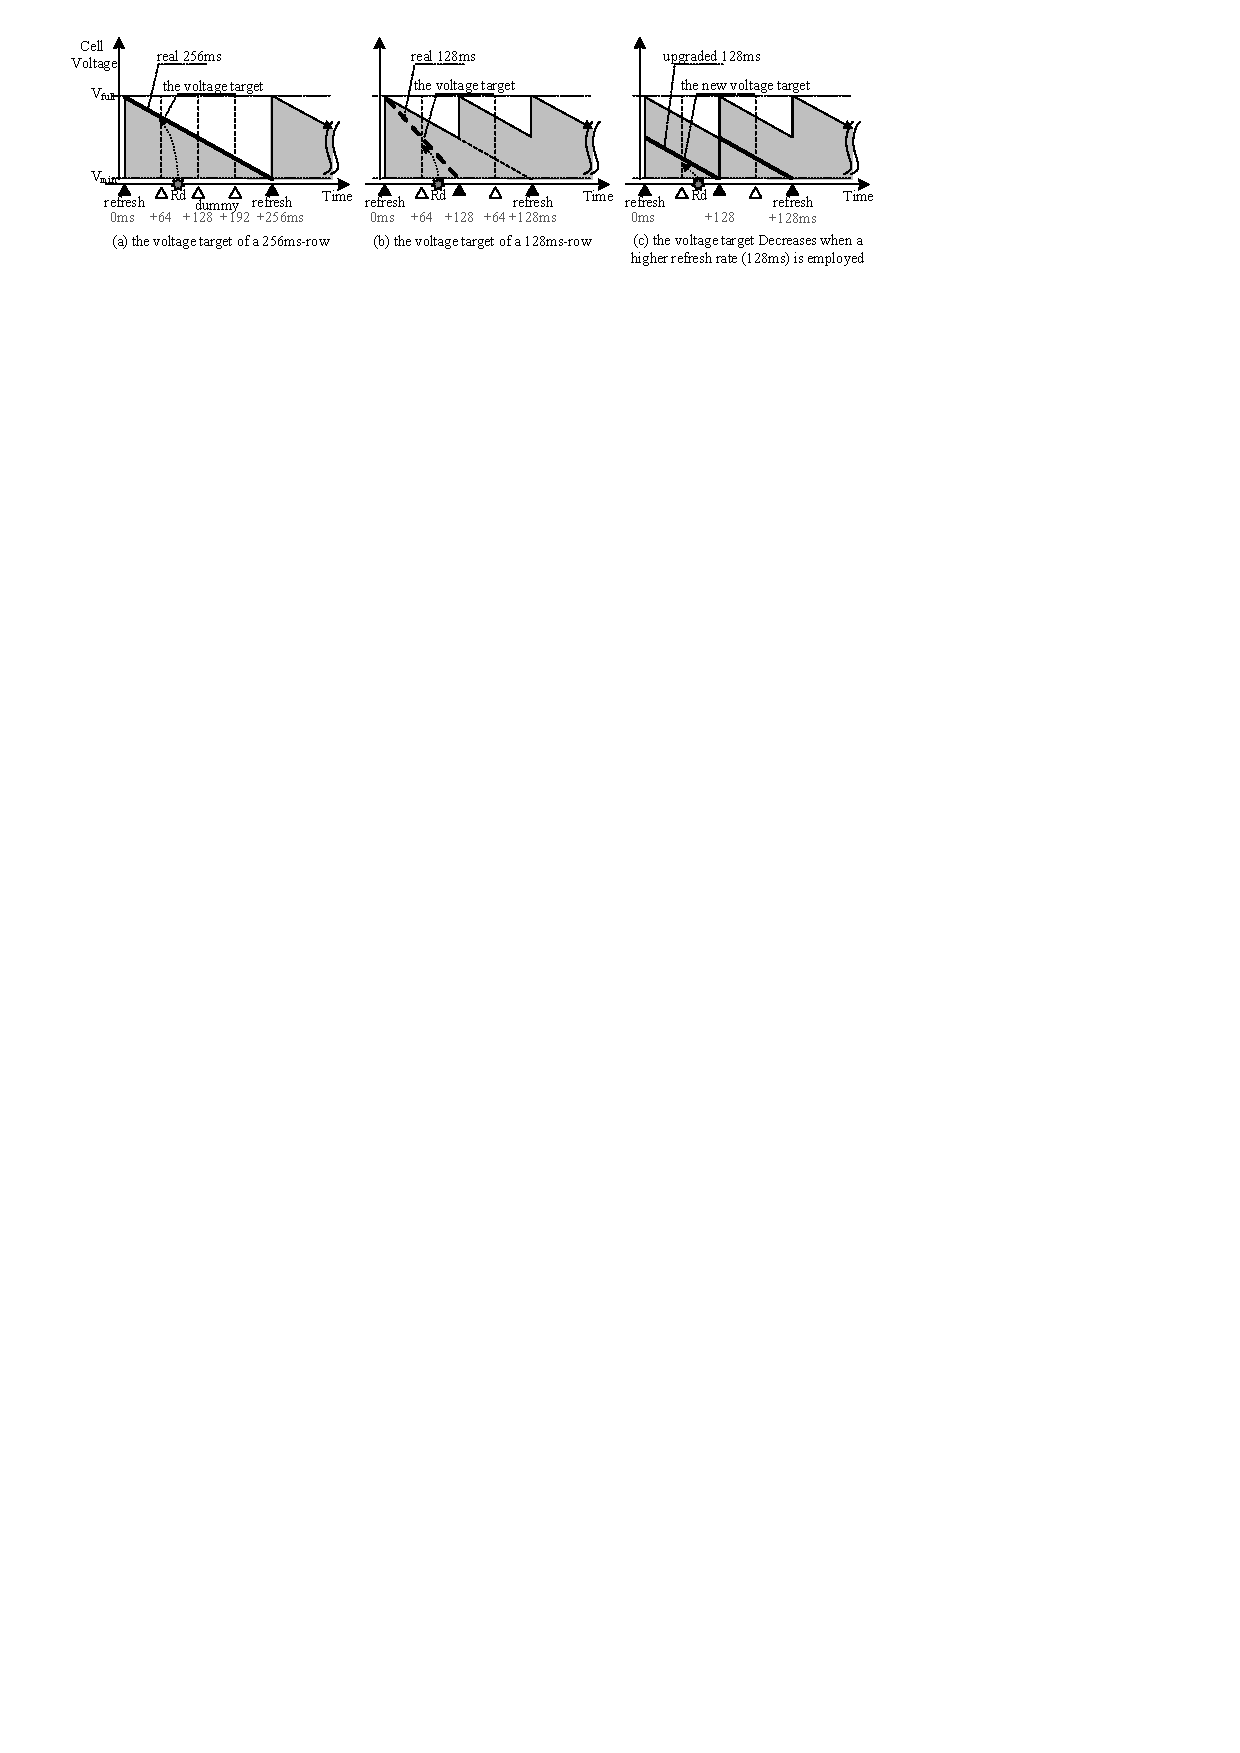
\includegraphics[width=6.4in]{figures/HPCA16/rt_selective.pdf}
\vspace{-0.2in}
\caption{The voltage target can be reduced if a strong row is refreshed at higher rate.}
\label{fig:rtselective}
\vspace{-0.3in}
\end{center}
\end{figure*}

Refreshing a 256ms-row at 128ms rate exposes more truncation benefits, as shown in 
Figure \ref{fig:rtselective}(c). For access "Rd'', it is sufficient to restore the voltage to 0.80V$_{dd}$ rather than 0.86V$_{dd}$ in above discussion. 
This is because a 256ms-row, even if being refreshed at 128ms rate, leaks slower than a real 128ms-row. We can adjust the timing values by following the solid thick line in \ref{fig:rtselective}(c), rather than the dashed thick line from a real 128ms-row, as shown in \ref{fig:rtselective}(b).
In particular, %as summarized in Table \ref{rt_selective_timing}, 
a row access, even if it is 128ms away from the next refresh to the row, just needs to restore the row to 0.86V$_{dd}$, rather than V$_{full}$ (=0.975V$_{dd}$) for a real 128ms-row. 

%\begin{table}[htbp]
%\vspace{-0.2in}
%\begin{center}
%\caption{Adjusted restore timing values in {\tt RT-select}}
%\vspace{-0.2in}
%\label{rt_selective_timing}
%\scalebox{0.7}
%{
%\begin{tabular}{|c||c|c|*3c|}
%\hline\hline
%Upgrade       &  Distance to Next  & Target restore      &{\tt tRAS}	  &{\tt tWR}	  &{\tt tRCD}\\
%              &  refresh           &  voltage (V$_{dd}$) &\multicolumn{3}{c|}{(DRAM cycles)} \\ \hline \hline
%256ms-$>$128ms  & [128ms, 64ms)      & 0.86 		&21		   &14	   	&15  \\ \cline{2-6}
%              & [64ms, 0ms)        & 0.80     &18      &11    	&15  \\ \hline \hline
%256ms-$>$64ms   & [64ms, 0ms)        & 0.80 		&18		   &11	   	&15  \\ \hline \hline
%128ms-$>$64ms   & [64ms, 32ms)        & 0.86 		&21		   &14	   	&15  \\ \cline{2-6} 
%			 & [32ms, 0ms)        & 0.80 		&18		   &11	   	&15  \\ \hline \hline 
%\end{tabular}
%}
%\end{center}
%\vspace{-0.1in}
%\end{table}

{\bf RT-select scheme.} 
While upgrading refresh rate reduces restore time, it generates more real refresh commands, which not only prolongs memory unavailable period but also consumes more refresh energy. 
Previous work shows that refresh may consume over 20\% of the total memory energy for a 32Gb DRAM device \cite{TC15:refresh, ISCA12:raidr}. Blindly upgrading the refresh rate of all rows is thus not desirable.

{\tt RT-select} upgrades the refresh rate of {\em selected bins}, those were touched, for {\em one refresh window}. It works as follows. 
A 3-bit rate flag is attached to each refresh bin to support multi-rate refresh. 
When there is a need to upgrade, e.g., from 256ms to 128ms rate, {\tt RT-select} updates the rate flag as shown in section~3.5, which converts the dummy refresh at +128ms in Figure~\ref{fig:rtselective}. 
A real refresh command rolls the rate back to its original rate, i.e., {\tt RT-select} only upgrades the touched bin for one refresh window, which incurs modest refreshing overhead to the system.

\section{Architectural Enhancements}

To enable {\tt RT-next} and {\tt RT-select}, we enhance the memory controller, as shown in Figure~\ref{fig:arch}. RT adds a truncation controller, to adjust the timing for read, write, and refresh accesses. This control is similar to past schemes that change timings \cite{HPCA13:tldram, ISCA13:charm, HPCA14:nuat}.  The memory controller has a register that records the next bin to be refreshed, referred to as {\tt Bin$_c$}, which rolls over every 64ms. 
It can also infer the mapping from row address to refresh bin, the same as that in \cite{ISCA15:reflex, ISCA14:disturbance}. 

To support multi-rate refresh, the memory controller keeps a small table that uses 3 bits to record the refresh rate of each refresh bin, similar to that in \cite{ISCA12:raidr, ISCA15:reflex}. As shown in Table \ref{tab:flag}, a 64ms-/128ms-/256ms- bin is set as `000'/`01A'/`1BC', respectively. Here `A' and `BC' are initialized to ones and decrement every 64ms.
While the refresh bin counter increments every in 7.8$\mu$s(=64ms/8192), a real {\tt REF} command is sent to refresh the corresponding bin only if its bin flag is `000', `010', or `100'. 
`A' and `BC' are changed back to `1' and `11' afterwards, respectively.

\begin{figure}[htbp]
\begin{center}
%\vspace{-0.1in}
\centering
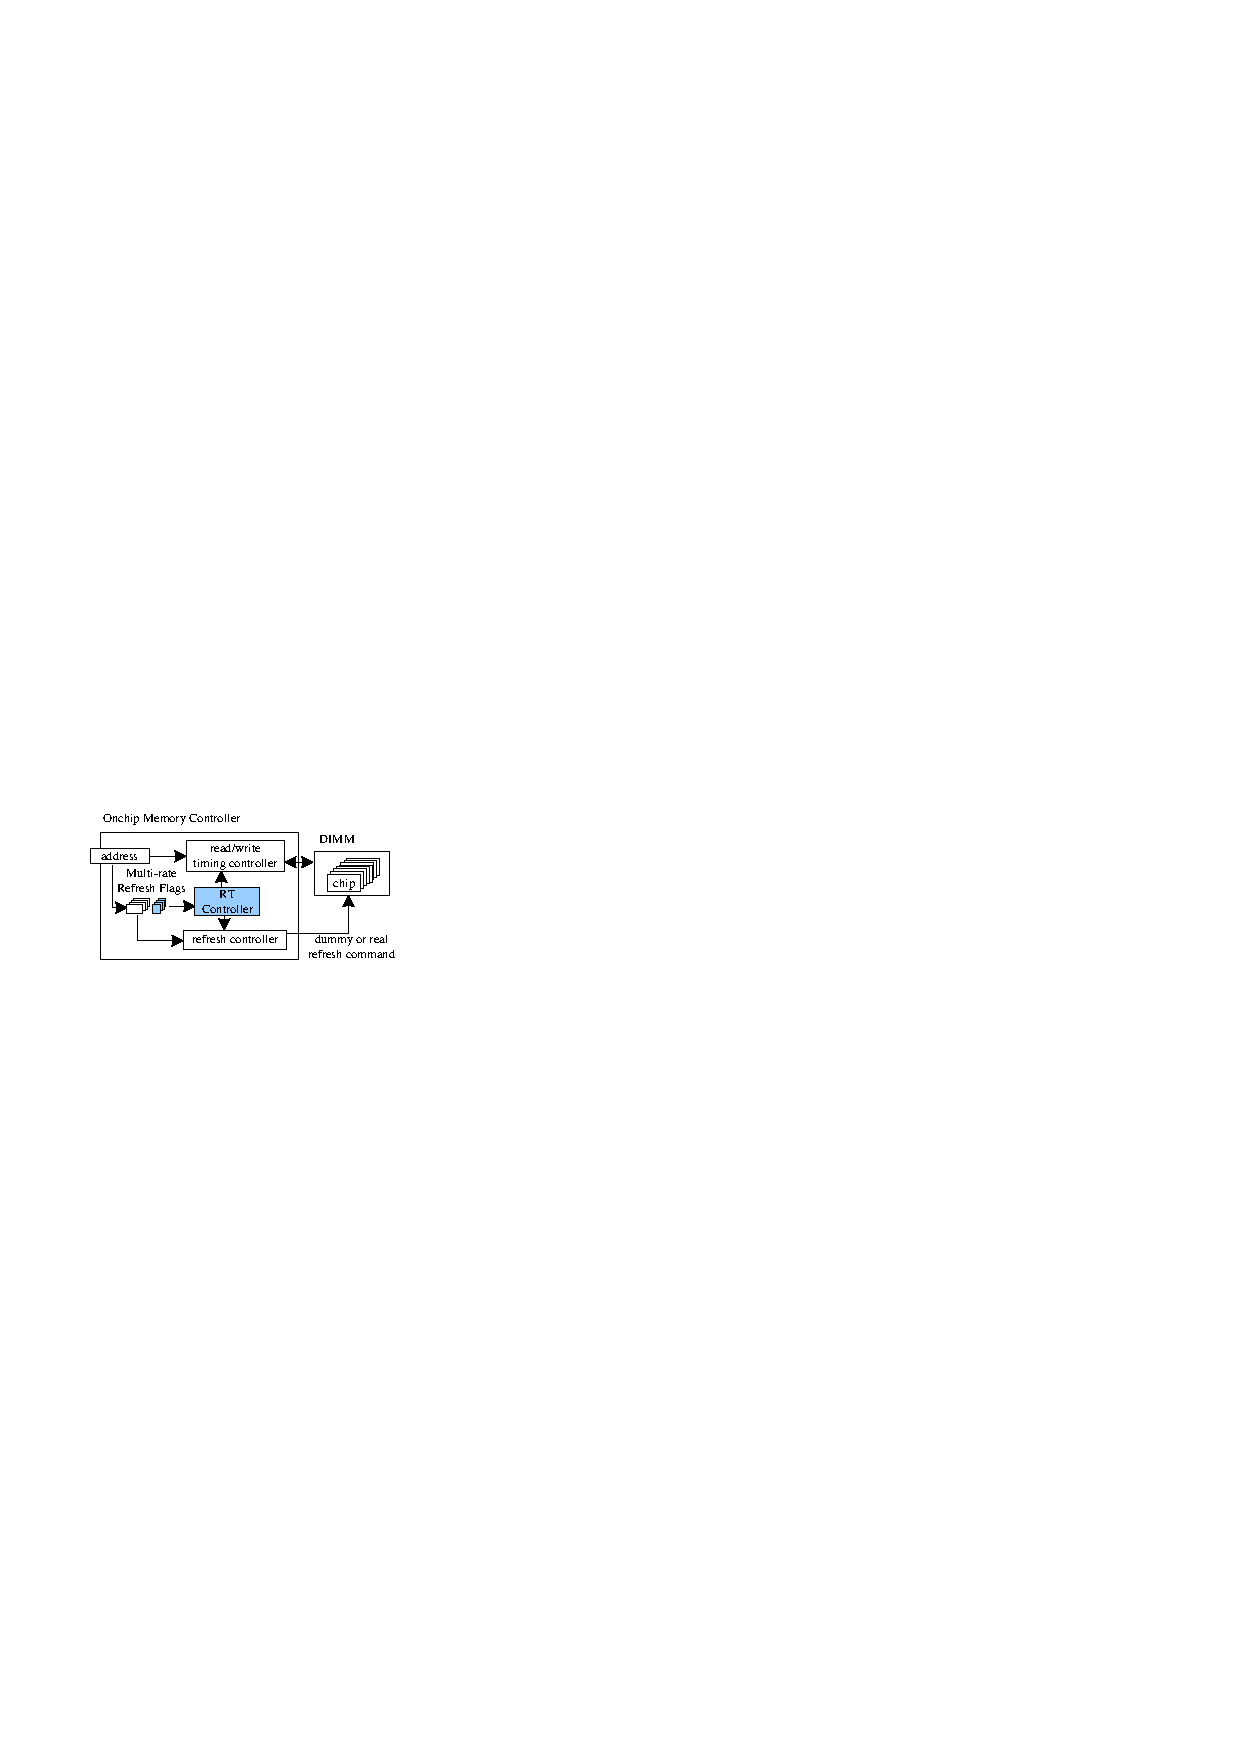
\includegraphics[width=3.25in]{figures/HPCA16/rt_arch.pdf}
\vspace{-0.1in}
\caption{The RT architecture (the shaded boxes are added components).}
\label{fig:arch}
\vspace{-0.45in}
\end{center}
\end{figure}

When upgrading the refresh rate of a refresh bin, we update the rate flag according to the last column in Table \ref{tab:flag}. For example, when upgrading a 128ms-bin to 64ms rate, we set the rate flag as `010', which triggers the refresh in the next 64ms duration and roll back to `011' afterwards. This effectively upgrades for one round. Upgrading 256ms-row to 128ms rate sets the flag as `1BC$\oplus$0B0', which always sets the middle bit to zero to ensure that the refresh distance is never beyond 128ms, and thus the sub-window can only be {\tt 3rd} and {\tt 4th} referring to Table \ref{rt_next_timing}. In general, the distance calculation in {\tt RT-select} is adjusted by adding further refresh rounds indicated by the two least significant bits (LSB) of rate flag.

 \begin{table}[htbp]
 \vspace{-0.25in}
\caption{Refresh rate adjustment table}
\vspace{-0.3in}
\begin{center}
\scalebox{0.8}
{
\begin{tabular}{l|l|l}
\hline \hline 
{Profiled refresh rate}	&{Rate flag}	&{Flag after rate upgrade}\\
\hline\hline
64ms		&$000$	& n/a\\
\hline
128ms		&$01A$	&128$\rightarrow$64ms: 010\\
\hline
256ms		&$1BC$	&256$\rightarrow$128ms: 1BC$\oplus$0B0\\
			&		&256$\rightarrow$64ms: 100\\
\hline\hline
\end{tabular}
}
\end{center}
\label{tab:flag}
%\vspace{-0.2in}
\end{table}

To enable multi-rate refresh, the %3KB (=3bits*8192) 
rate table is accessed before each refresh to determine if a real or dummy command should be sent. To enable {\tt RT-select}, the rate table is also 
accessed before each memory access to decide the refresh distance, and then to complete the upgrade after the access.
%accessed before each memory access to decide if it is necessary to upgrade the rate. 
The extra energy is minimal, as shown in Section~\ref{subsec:energy}.

\section{Experimental Methodology}\label{sec:experiment}
\subsection{Configuration}\label{subsec:setting}
To evaluate the effectiveness of our proposed designs, we performed the simulation using the memory system simulator USIMM \cite{SIMU:usimm}, which simulates DRAM system with detailed timing constraints. 
USIMM was modified to conduct a detailed study of refresh and restore operations.

We simulated a quad-core system with settings listed in Table \ref{tab:configuration}, similar to those in \cite{HPCA13:refresh_pausing, HPCA14:nuat}. 
The DRAM timing constraints follow Micron DDR3 SDRAM data sheet \cite{SIMU:datasheet}. By default, DRAM devices are refreshed with 8K {\tt REF} within 64ms, and {\tt tRFC} is 208 DRAM cycles, which translates into a {\tt tREFI} of 7.8 $\mu$s (i.e., 6240 DRAM cycles). As  \cite{HPCA13:refresh_pausing}, the baseline adopts closed page policy, which works better in multicore systems \cite{PACT12:close_page}. 

\begin{table}[htbp]
\vspace{-0.2in}
\caption{System Configuration}
\vspace{-0.3in}
\begin{center}
\scalebox{0.8}
{
\begin{tabular}{l|l}
\hline\hline
Processor			&four 3.2Ghz cores; 128 ROB size\\
				&Fetch width: 4, Retire width: 2, Pipeline depth: 10\\
\hline
				&Bus frequency: 800 MHz\\
 				&Write queue capacity: 64\\
Memory			&Write queue watermarks: 40/20\\	
Controller			&Address mapping: rw:cl:rk:bk:ch:offset\\
				&Page management policy: close-page with FRFCFS\\

\hline
				&2channels, 1rank/channel, 8banks/rank, \\
DRAM			&64K rows/bank, 8KB/row, 64B cache line\\
				&tCK=1.25ns, width: x8\\
%DRAM			%&tCAS(CL): 13.75ns, tRCD: 13.75ns, tRC: 48.75ns\\
				%&tCWD: 6.25ns (5 cycles), tBURST: 5.0ns (4 cycles)\\
				%&tRAS: 35ns, tRP: 13.75ns, tFAW: 24 cycles,\\
				%&tRRD: 5 cycles, tRFC: 208nCK, tREFI: 7.8$\mu$s\\
\hline\hline

\end{tabular}
}
\end{center}
\label{tab:configuration}
\vspace{-0.4in}
\end{table}

\subsection{Workloads}
For evaluation, we use workloads from the Memory Scheduling Championship \cite{SIMU:msc}, which covers a wide variety of benchmarks, including five commercial applications \textit{comm1} to \textit{comm5}, nine benchmarks from PARSEC suite and two benchmarks each from the SPEC suite and the Biobench suite. Among them, \textit{MT-fluid} and \textit{MT-canneal} are two multithreaded workloads.
As \cite{HPCA13:refresh_pausing}, the benchmarks are executed in rate mode, and the time to finish the last benchmark is computed as the execution time.


\section{Results}\label{sec:results}

%\subsection{Schemes to Study}
We evaluated our proposed RT schemes on system performance, memory access latency and energy, and then studied their sensitivities to different configurations.
To study different aspects of RT, we analyze different set of schemes in each figure.

\subsection{Impact on Performance}

Figure \ref{fig:time} compares the execution time of different schemes.
The results are normalized to \texttt{Baseline}. 
In the figure, {\tt Gmean} is the geometric mean of the results of all workloads.

\begin{figure*}[htbp] 
\centering
\centering
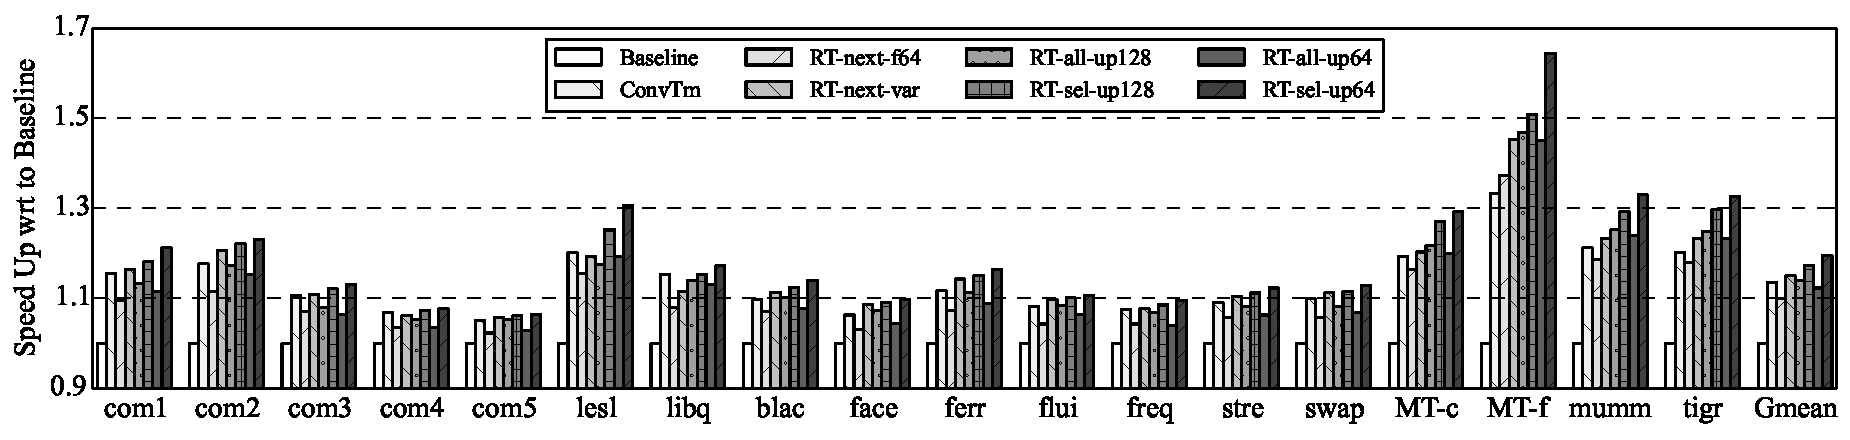
\includegraphics[width=6.5in]{{figures/HPCA16/DATA/0903.dat/4Gb/stat_4Gb_Cycles.perc.main.dat}.pdf}
\vspace{-0.45in}
\caption{Performance comparison of different schemes. {\tt Baseline} and {\tt ConvTm} adopts projected and conventional timings, respectively; {\tt NoRefresh} assumes no refresh activity in {\tt Baseline}; {\tt RT-next-XX} truncates restore based on its distance to next fresh, and {\tt f64} and {\tt var} supports fixed 64ms refresh rate and multiple rates, respectively; {\tt RT-all-upYY} aggressively upgrades refresh bins with rates lower than {\tt YY} to {\tt YY}; finally, {\tt RT-sel-upYY} are optimized schemes to balance the restore benefits and refresh overhead.}
\label{fig:time}
\vspace{-0.45in}
\end{figure*}

On average, \texttt{RT-next-f64} achieves 10\% improvement over {\tt Baseline} by truncating restore time. {\tt RT-next-var} identifies more truncation opportunities in multi-rate refresh DRAM modules and achieves better, i.e., 15\%, improvement. 
While {\tt RT-all-up128} truncates more restore time through refresh rate upgrade, it introduces extra refresh overhead and thus is slightly worse than {\tt RT-next-var}.
\texttt{RT-sel-up128} achieves 2.4\% improvement over \texttt{RT-next-var}
by balancing refresh operations and restore benefits. 
The performance gap between upgrading all rows and selective upgrading is even larger when we aggressively upgrade refresh rate to 64ms. \texttt{RT-sel-up64} achieves the best performance --- it is 19.5\% speedup over {\tt Baseline}, or 4.5\% better than \texttt{RT-next-var}.
The performance trend across the schemes demonstrates that our restoring schemes achieves a good balance between refresh and restore.

%Generally, memory access intensive workloads such as \textit{com1}, \textit{libq} and \textit{mumm} benefit most from the reduced restore timing.
%Particularly, \textit{MT-f} obtains the largest performance improvement because of the parallel access patterns and relatively tight gaps between accesses, which greatly enlarges the effect of shortened {\tt RAS} and {\tt WR}.

\subsection{Energy Consumption}\label{subsec:energy}
Figure \ref{fig:energy} compares the energy consumption of different schemes. 
We reported the energy consumption breakdown ---  background ({\tt bg}), activate/precharge ({\tt act/pre}), read/write ({\tt rd/wr}) and refresh ({\tt ref}). We summarized the results according to benchmark suites, where results are averaged over workloads within each suite.
We used the Micron power equations \cite{TOOL:power}, and the parameters from vendor data sheets \cite{SIMU:datasheet} with scaling. 

To enable truncation in multi-rate refresh DRAM modules, we need to query the refresh rate for each access. The refresh rates for 8192 bins are organized as 3KB direct mapped cache with 8B line size. We used CACTI5.3 \cite{URL:cacti} to model the cache with 32nm technology --- it requires 0.22ns access time, occupies 0.02mm$^2$ area, consumes 1.47mW standby leakage power, and spends 3.33pJ energy per access. The extra energy is trivial (less than 0.5\%) and is reported together with {\tt bg}. 

\begin{figure}[htbp] 
%\vspace{-0.1in}
\begin{center}
\centering
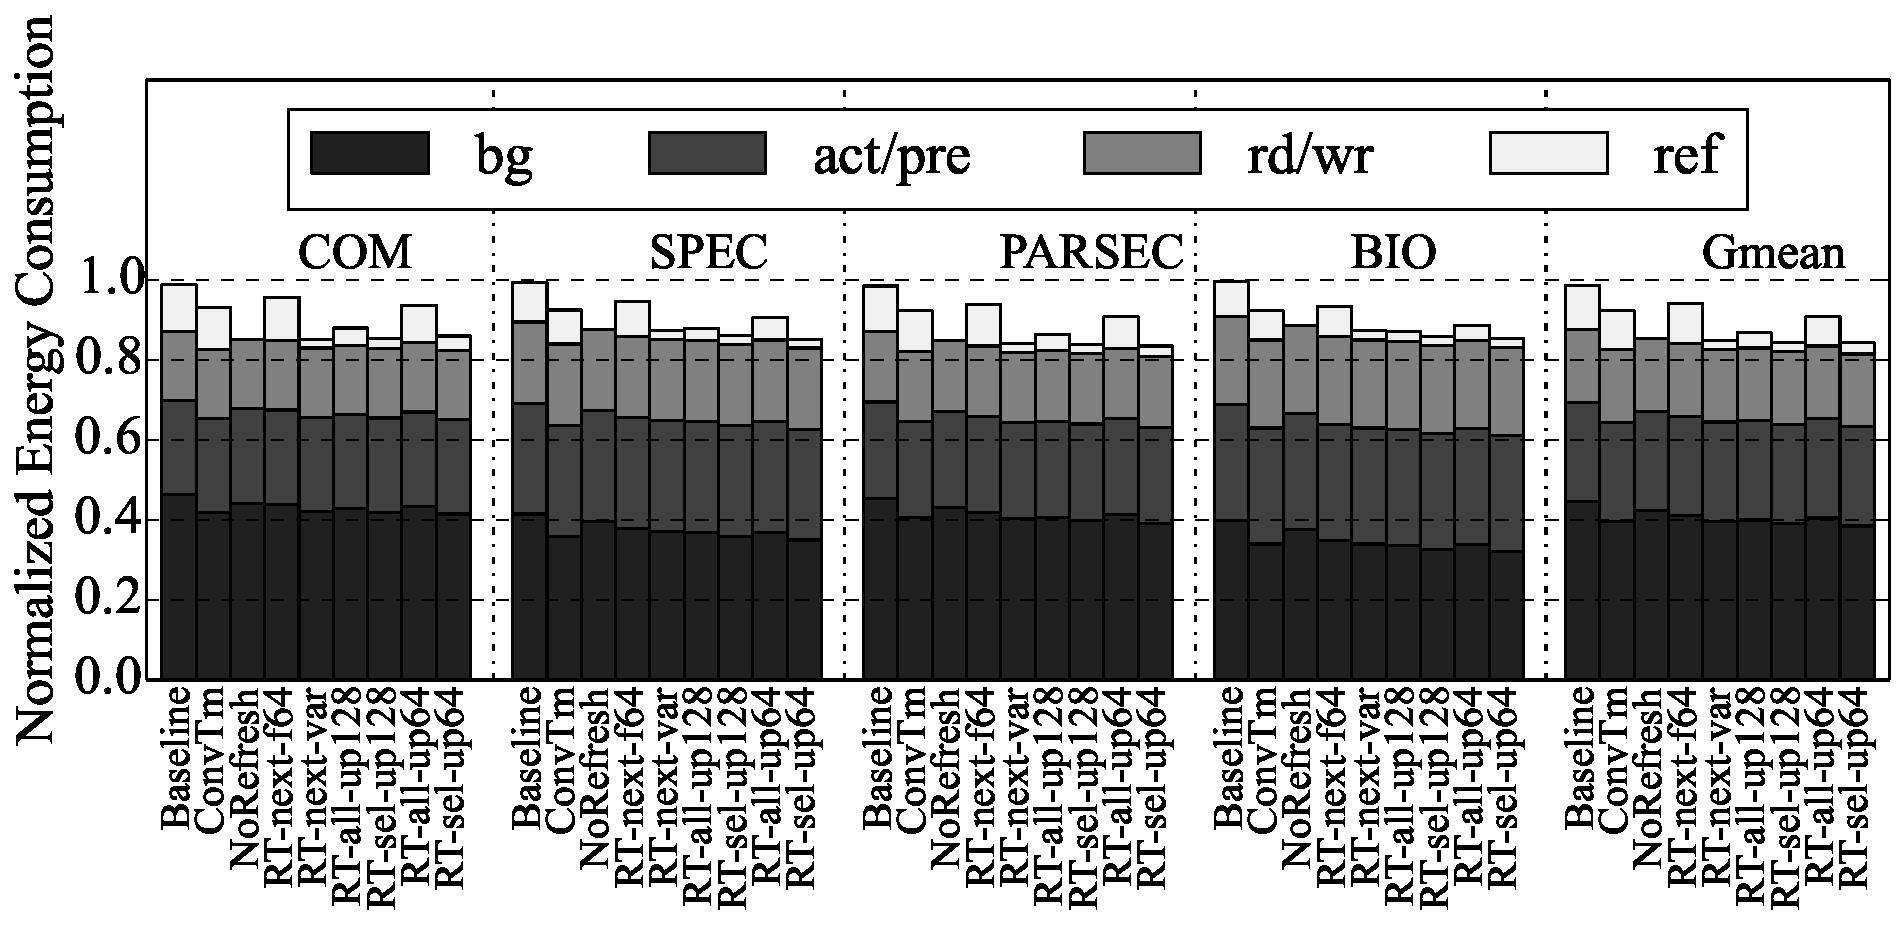
\includegraphics[width=0.7\textwidth]{{figures/HPCA16/DATA/0903.dat/4Gb/stat_4Gb_energy.all.dat.cat}.pdf}
\vspace{-0.1in}
\caption{Comparison of memory system energy.}
\label{fig:energy}
\end{center}
\vspace{-0.4in}
\end{figure}

From the figure, we observed that the device refresh energy for 4Gb chips is small. 
Due to increased refresh operations, {\tt RT-all-up128/-up64} consume much more refresh energy than {\tt RT-all-up128/-up64}, respectively. \texttt{RT-sel-up64} saves 17\% energy compared to {\tt Baseline}, and consumes slightly lower energy than \texttt{NoRerefresh} due to decreased execution time. And, as expected, {\tt RT-sel-} refresh schemes is more energy efficient than {\tt RT-all-} refresh peers.


\subsection{Comparison against the State-of-the-art}
Figure \ref{fig:state} compares RT with three related schemes in the literature. 
\begin{itemize}
\itemsep -1pt
\item
{\tt Archshield+} implements a scheme that treats all the cells with long restore latency as failures and adopts Archshield \cite{ISCA13:archshield} to rescue them. 
\item
{\tt MCR} is the recently proposed scheme that trade DRAM capacity for better timing parameters \cite{ISCA15:mcr}. {\tt $2x$ MCR} and {\tt $4x$ MCR} are the two options that reduce DRAM capacity to 50\% and 25\% of the original, respectively.
\item
{\tt ChunkRemap} implements the scheme that differentiates chunk level restore difference and constructs fast logic chunks through chunk remapping \cite{DATE15:twr}. 

\end{itemize}

\begin{figure}[htbp] 
\begin{center}
\centering
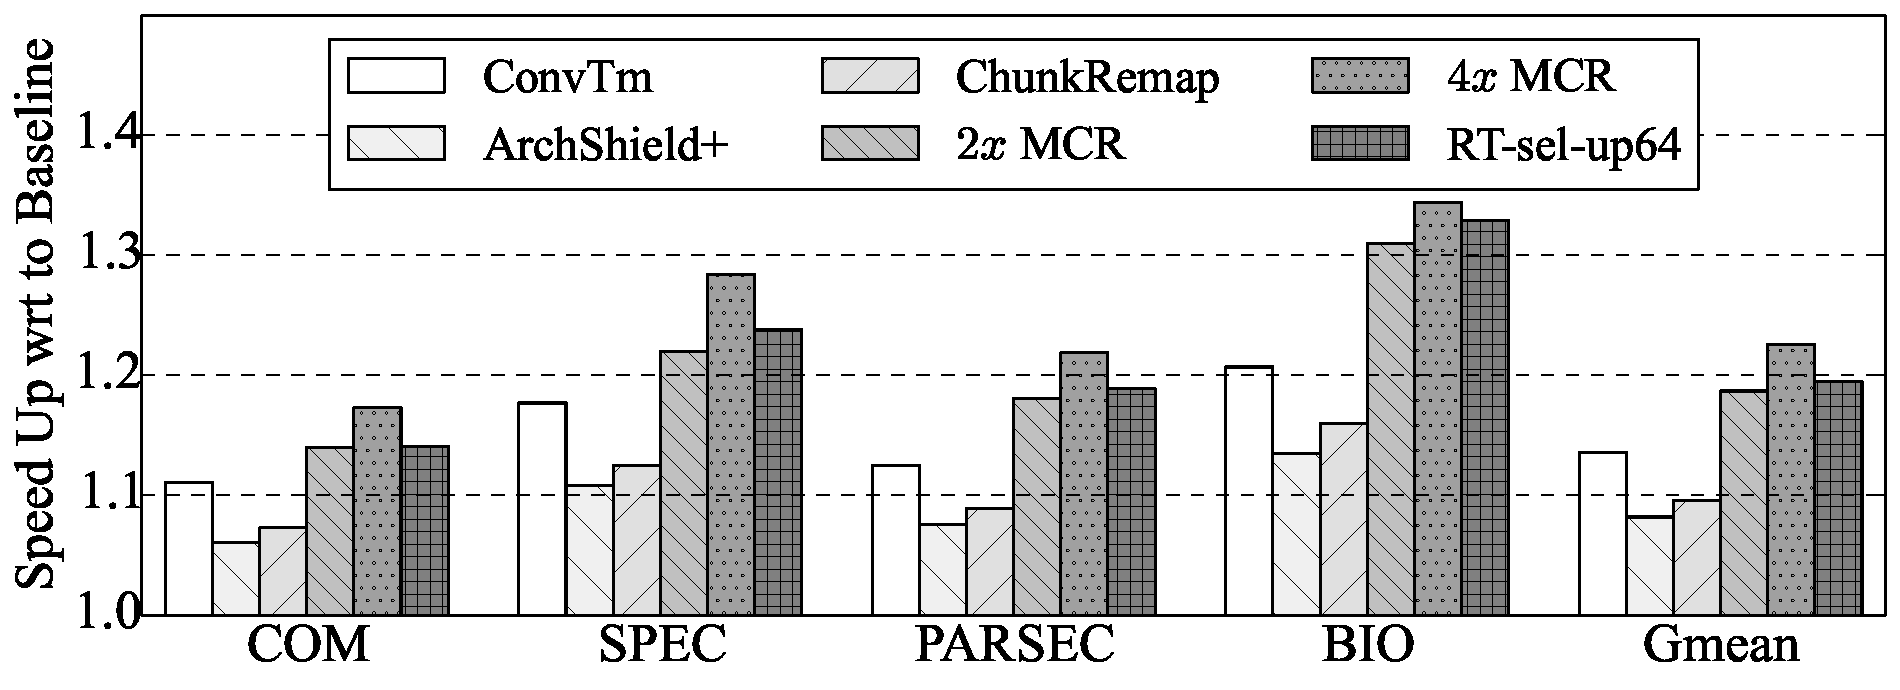
\includegraphics[width=3.4in]{{figures/HPCA16/DATA/0903.dat/4Gb/stat_4Gb_Cycles.perc.statart.dat}.pdf}
\vspace{-0.2in}
\caption{Comparison against the state-of-the-art.}
\label{fig:state}
\vspace{-0.45in}
\end{center}
\end{figure}

The figure shows that {\tt Archshield+} and {\tt ChunkRemap} are approaching {\tt ConvTm} while {\tt RT-sel-up64} is 5.2\% better than {\tt ConvTm}, exploiting more benefits from reduced restore time.
{\tt $4x$ MCR} outperforms {\tt RT-sel-up64} by a modest percentage, and {\tt RT-sel-up64} works better than {\tt $2x$ MCR}.

{\tt MCR} shares similarity with {\tt RT-select}, i.e., we share the observation that a line that is refreshed more frequently can be restored to a storage level lower than V$_{full}$. {\tt MCR} exploits this with significant DRAM capacity reduction while {\tt RT-select} takes a light weight design that upgrades used bins only for one refresh window, and leaves all the other bins being refreshed at original rates. 

%From the figure, {\tt $4x$ MCR} outperforms {\tt RT-sel-up64} by a modest percentage. 
%This is because {\tt MCR} improves the baseline by reducing not only restore time but also sensing time while {\tt RT-sel-up64} focuses only restore time. 
%{\tt RT-sel-up64} works better than {\tt $2x$ MCR} because it upgrades the refresh rate of a bin for one refresh window at a time, which significantly reduces refresh overhead (as shown with the difference from {\tt RT-all-up64}). 



%By focusing on restoring and respecting the DRAM auto-refresh, we only improve tRAS and tWR in this paper, whereas {\t MCR} reduces both tRCD and tRFC besides tRAS \footnote{Although {\tt MCR} \cite{ISCA15:mcr} failed to take write restoring (tWR) into account in the paper, for a fair comparison, we embed tWR reductions into MCR schemes.}
%. 
%Nevertheless, the figure shows that our proposed {\tt RT-sel-up64} outperforms {\tt MCR-2} and approaches {\tt MCR-4} (the gap is within 3\%).
%The performance difference is pretty narrow because: (1) our RT schemes take use of the multi-rate refresh to do restoring, which is capable to achieve restoring reduction and refresh improvement simultaneously comparing to {\tt Baseline}; to the contrary, {\tt MCR} ignored the retention time variation to use a fixed 64ms refresh rate; (2) RT schemes combines distance-aware restore and refresh rate upgrade, which makes the best timing values outperform those can be achieved by {\tt MCR}.


\begin{table}[htbp]
\vspace{-0.2in}
\caption{Comparing EDP between RT and MCR (lower is better).}
\vspace{-0.3in}
\begin{center}
\scalebox{0.8}
{
\begin{tabular}{*5c}
\hline\hline
Cases		& {\tt ConvTm} & {\tt RT-sel-up64}	& {\tt $2x$ MCR}	&{\tt$4x$ MCR-4}\\
\hline
\texttt{Same Chip}	& 1.0$\times$ &0.715$\times$		&0.753$\times$		&0.713$\times$\\
\texttt{Same Capacity}	& 1.0$\times$  &0.715$\times$		&0.918$\times$		&1.068$\times$\\
\hline\hline

\end{tabular}
}
\end{center}
\label{tab:edp}
\vspace{-0.45in}
\end{table}

Given that {\tt MCR} improves performance at a significant capacity reduction.
We next comparing the energy-delay-product (EDP) --- ``Same Chip'' is optimistic assumption as {\tt $4x$ MCR} has only 25\% available capacity, which is likely to have more page faults in practice. ``Same capacity'' enlarges the raw chip in {\tt MCR} by two/four times, which introduces more background power. {\tt RT-sel-up64} shows good potential as its EDP closely matches that of {\tt MCR} under ``same chip'' setting, and is much better under ``same capacity'' setting.

 
%Note that performance improvement of {\tt MCR} is resulted from a serious capacity effectiveness loss. For {\tt MCR-4}, four rows are formed as a group and only one row can function at a time, and thus 75\% capacity becomes unavailable. And thus, devices should be enlarged by four times to avoid frequent page fault. Further, we conservatively assume that in larger chips, all powers except {\tt bg} stay the same as 4Gb-chip.

%From Table \ref{tab:edp}, we can see that for the scenario of same overall capacity using 4Gb-chip, which may introduce substantial page fault overhead, {\tt RT-sel-up64} achieves a better EDP than {\tt MCR-2}, and vey close to {\tt MCR-4}. The explanation is that despite that {\tt MCR-4} has a better performance, its refresh energy is significantly higher than that of {\tt RT-sel-up64} and thus the EDP gets almost the same. However, for same effective capacity, 8Gb-/16Gb-chip is used for {\tt MCR-2} and {\tt MCR-2}, {\tt RT-sel-up64} shows a much lower EDP.

\subsection{Further Studies}
\label{SEC:ideal_comp}
To further evaluate the effectiveness of RT, we compare against several \textit{ideal} schemes, including refresh-free scheme, conventional timings and best interval timings, etc. The results show that RT schemes defeat all of those schemes and the gap to the most ideal scheme of \textit{best interval without refresh} is within 3\%.

In addition, we evaluate the performance sensitivity by varying configurations including chip density, refresh granularity, refresh sub-window and page management policy. The results positively demonstrate the robustness of the achieved performance.

\section{Conclusion}\label{sec:conclusion}
In this paper, we studied the restoring issues in further scaling DRAM, identified partial restore opportunity and proposed two restore truncation (RT) schemes to exploit the opportunities with different tradeoffs. Our experimental results showed that, on average, RT improves performance by 19.5\% and reduces  energy consumption by 17\%.


\chapter{Further Explorations of Restoring}
\label{chapter:future_study}
This chapter will briefly discuss further explorations of restoring, as future work. We'll extend the restoring topic to approximate computing, memory information leakage and 3D stacked memory.

\section{Combine Restoring with Approximate Computing} \label{work:approx}
\subsection{Introduction on Approximate Computing}
Energy and power are increasing concerns in nowadays computer systems, ranging from mobile devices to data centers; and much energy is spent on guaranteeing correctness \cite{PLDI11:enerj}.
Nevertheless, many modern applications have intrinsic tolerance to inaccuracy \cite{ISCA10:relax, PLDI11:enerj}. For instance, lots of problems have no perfect answer in domains like machine learning, computer vision and sensor data analysis, and hence the adopted solutions rely on heuristic approach; and, large-scale data analytics cares more about aggregate trends rather than the correctness of individual data elements. Apparently, these applications provide good opportunities to explore energy-accuracy tradeoff.

Approximate computing necessitates the collaboration of different layers spanning circuits, architectures and algorithms. On program level, we should annotate the approximate data, which is non-critical and able to tolerate inexactness; on instruction level, the system should distinguish approximate and precise instructions and then take use of different strategies to execute; the fundamental energy savings rely on hardware techniques, including voltage reduction, floating point rounding and refresh rate reduction, etc.

To quantify the energy-accuracy tradeoff, we need to measure the output quality of approximate execution and should ensure that the quality loss is sustainable.
The qualify-of-service (QoS) metrics are per-application specific, and are measured by comparing the final outputs of approximate execution against those of precise one.
For instance, if the outputs are images, then the QoS can be evaluated as the average difference of per-RGB value \cite{PLDI11:enerj} between the executions.

\subsection{Related Work}
Prior works on approximate computing performed explorations from both hardware \cite{DATE06:cmos, DATE10:proc, ISCA10:relax, ASPLOS11:flikker, ASPLOS12:disciplined, MICRO12:neural, MICRO13:appro, MICRO14:appro, MICRO15:doppelganger} and software \cite{PLDI10:green, PLDI11:enerj, ASPLOS11:knob, OOPSLA15:topaz}. Among them, there is significant research on storing approximate data more efficiently, which is also the focus of our tentative exploration.
Flikker \cite{ASPLOS11:flikker} refreshes approximate data at lower rates to save DRAM refresh energy, which is recently extended by \cite{MEM14:sparkk, CASES15:appro}.
\citeN{ASPLOS12:disciplined} proposed to apply dual voltage to SRAM array to balance energy and accuracy; Drowsy caches \cite{ISCA02:drowsy} reduces the supply voltage to save power; to improve PCM's lifetime and performance, \cite{MICRO13:appro} proposed to reduce write precision and reuse failed cells.

\subsection{General Ideas}
According to the observations of our prior studies \cite{DATE15:twr}, whereas the worst-case {\tt tWR} of the whole memory suffers from significant increase, a large portion of cells have {\tt tWR} within the specification range.
Such variation provides opportunity for applying approximate computing to achieve performance and performance improvements: {\tt tWR} can be aggressively reduced to low value(s) as long as we can guarantee the correctness of precise data, and control the error impact of approximate data.

Program annotation can be performed by inserting assembly code, which will be identified by Pintool. Pintool simulates the real instruction execution, and when stepping into annotated approximate region, it injects errors using the underlying DRAM bit mask.
As prior arts \cite{PLDI11:enerj, MICRO14:appro}, we will control the annotation to let the program run to the end, and compare the approximate results against precise ones to report QoS. Simultaneously, Pintool outputs memory accesses, which are then fed into conventional memory simulator to collect performance and energy values. The most challenging part lies on the tradeoff between QoS and performance achievement: fine-grained and aggressive {\tt tWR} control benefits memory performance, but is likely to introduce too many errors. We will take some measurements to constraint the errors, candidate solutions can be dedicated allocation, location correction or memory bit remapping, etc.

%\begin{itemize}
%\itemsep 0pt
%\item Fixed tWR, e.g., 15, and then do mapping or correction
%\item Random mapping, apply full tWR for precise data
%\end{itemize}

\section{Study Security Issues of Restoring Variation} \label{work:security}
%\subsection{Introduction on Memory Security Issues}
Modern computing systems suffer from increasing concerns on privacy, security and trust issues, with timing channel attacks as a representative example.
And recently, the concern on timing channel attack has moved from shared caches \cite{BSDCan05:cache_fun, ISCA07:cache_channel, HASP13:cache} and on-chip networks \cite{NOCS12:noc_channel, ISCA13:surfnoc} to shared main memory \cite{CCS13:oram, HPCA14:channel, MICRO15:fs}.
Memory access pattern can leak a significant amount of sensitive information through statistical inference \cite{CCS13:oram}.

As a remedy, ORAM \cite{CCS13:oram} was proposed to conceal a client's access pattern to remote storage by continuously shuffling and re-encrypting data as they are accessed.
\citeN{HPCA14:channel} proposed temporal partitioning (TP) to isolate thread accesses to hide access pattern. As an improvement, Fixed Service (FS) policies were studied by \cite{MICRO15:fs} to reshape memory access behaviors without much performance degradation.

Compared to the simple case of a single set of timings for the whole memory system, restoring variations in further scaling DRAM are likely to leak more information. For instance, various memory access speeds to different memory regions may expose the footprint to malicious users. And things can be much worse with the adoption of NUMA-aware page allocation and approximate computing. The former easily leak the frequently accessed data, and the latter correlates data to its location origin \cite{ISCA15:prob}. 

In addition, simply borrowing the schemes in \cite{HPCA14:channel, MICRO15:fs} would introduce higher overhead because of the much longer worst-case restoring timings.
As a result, it is necessary to integrate information leakage, restoring issues, page allocation and approximate computing to come out a workable solution with acceptable performance loss and safety guarantee.


%\subsection{Related Work}

%\subsection{Motivations and Proposed Ideas}

\section{Explore Restoring in 3D Stacked DRAM} \label{work:stacked}
Recent advances in die stacking techniques enables efficient integration of logic and memory dies in a single package, with a concrete example of Hybrid Memory Cube \cite{HMC:spec2}.
HMC is especially promising for its innovative architecture that stacks multiple memory dies atop of the bottom logic die, and adopts packetized serial link interface to transfer data and requests \cite{ICCD15:dlb}.
With the superior high bandwidth, low latency and packet-based interface, lots of work have proposed to move computation units inside the logic die \cite{JMicro:ndp, ISCA15:pim}.
However, thermal management is a big issue in stacked memories \cite{DAC06:3dmodel, WONDP14:thermal}, and the deployment of bottom computation logics like simple cores \cite{ISCA15:pim} and even GPU \cite{HPDC14:pim_gpu} worsens the issue. Besides, temperature variations exist among vertical dies \cite{ICCD13:temp}. It is known that DRAM is sensitive to temperature changes, including refresh \cite{HPCA15:al-dram, ISCA13:ddr4} and restoring time \cite{PATENT14:twr, MEM14:twr}.
Therefore, it is worthwhile to explore restoring time in stacked memories, and utilize the temperature characteristics to dig more opportunities to boost performance. 

%\subsection{Introduction on Stacked DRAM}

%\subsection{Related Work}

%\subsection{Motivations and Proposed Ideas}

\chapter{TIMELINE OF PROPOSED WORK}
\label{chapter:timeline}
\begin{table}[ht]
\vspace{-0.3in}
\caption{Timeline of Proposed Work.}
\vspace{-0.15in}
\centering
\scalebox{0.85}
{
\begin{tabular}{|l|l|l|}
\hline
\textbf{Date} & \textbf{Content} & \textbf{Deliverable results} \\
\hline
Jan - Feb  & Explore restoring in approximate computing & Pin-based framework for \\
 & in Section \ref{work:approx} of Chapter \ref{chapter:future_study}& restoring approximation \\
\hline
Mar - May  & Integrate restoring with information leakage & Experimental data of memory\\% through access pattern &  Paper submission \\
 & in Section \ref{work:security} of Chapter \ref{chapter:future_study}& performance and security\\
\hline
Jun - Sep & Study restoring in Hybrid Memory Cube (HMC) & Modified simulator of temperature\\
 & in Section \ref{work:stacked} of Chapter \ref{chapter:future_study}&  effect of restoring in HMC \\
\hline
Jul - Oct  & Thesis writing & Thesis ready for defense \\
\hline
Oct - Dec & Thesis revising & Completed thesis \\
\hline
\end{tabular}
}
\label{tab:timeline}
\end{table}

The proposed works will be undertaken as shown in the Table \ref{tab:timeline}.
I will start the effort with task (1) to develop Pin-based framework for approximate computing of restoring. This task involves program annotation, chip generation, QoS evaluation, and conventional performance simulation, etc.
While multiple complicated subtasks are there, this task has been partially finished, and will not take much time to complete.
Afterwards, I'll move to task (2) to study information leakage in restoring scenario, and this task is partially on basis of the previous approximation work.
With the completion of task (2), the overall goal of exploring DRAM restoring in application level have been reached, and then I'll start the study restoring's temperature effect in HMC, i.e., task (3).
The general infrastructure can be borrowed from my previous HMC work \cite{ICCD15:dlb}. This task might be performed concurrently with other jobs, and thus might take more time to finish.
At the end of task (3), the holistic exploration of DRAM restoring is considered finished, and thus I'll summarize all the tasks into my final thesis.

\chapter{SUMMARY}
\label{chapter:summary}
\begin{table}[ht]
\vspace{-0.3in}
\caption{Timeline of Proposed Work.}
\vspace{-0.15in}
\centering
\scalebox{0.85}
{
\begin{tabular}{|l|l|l|}
\hline
\textbf{Date} & \textbf{Content} & \textbf{Deliverable results} \\
\hline
Sep.-   & Explore restoring in approximate computing & Pin-based framework for \\
 & in Section \ref{work:approx} of Chapter \ref{chapter:future_study}& restoring approximation \\
\hline
Mar - May  & Integrate restoring with information leakage & Experimental data of memory\\% through access pattern &  Paper submission \\
 & in Section \ref{work:security} of Chapter \ref{chapter:future_study}& performance and security\\
\hline
Jun - Sep & Study restoring in Hybrid Memory Cube (HMC) & Modified simulator of temperature\\
 & in Section \ref{work:stacked} of Chapter \ref{chapter:future_study}&  effect of restoring in HMC \\
\hline
Jul - Oct  & Thesis writing & Thesis ready for defense \\
\hline
Oct - Dec & Thesis revising & Completed thesis \\
\hline
\end{tabular}
}
\label{tab:timeline}
\end{table}





Current fault tolerance approaches rely exclusively on either time or hardware redundancy to hide failures from being seen by users. 
Rollback recovery, which exploits time redundancy, requires full or partial re-execution when failure occurs.  
Such an approach
can incur a significant delay, % subjecting cloud service providers to SLA violations,
and high power costs due to extended execution time.
On the other hand, Process Replication relies on hardware redundancy and executes multiple
instances of the same task in parallel to guarantee completion with minimal delay. 
This solution, however, requires a significant increase in hardware resources and increases the power consumption proportionally. 


\appendix                      
%After this command, chapters will be formatted as appendices. For example
%\chapter{Possible Appendix}
%\label{appendix:effectEventInferenceRules}
%\input{appendixEffectEventInference}

%\chapter*{BIB}
\begin{singlespace}
%\nocite{*}
%\renewcommand{\bibsection}{} %remove automatically generated title, like "REFERENCE" or "BIBLIGROPHY"
\bibliographystyle{plainnat}
{
\footnotesize
\bibliography{references/refresh,references/twr,references/scaling,references/jedec,references/dram,references/approx_security,references/stacked,references/page_os,references/hpca16}
}
\end{singlespace}
%\bibliography{gfbf,sentiment,agreementStudy,effectEventCorpus,effectEventInference,generalEventCorpus,generalEventInference,myWork}          %\safebibliography is used the same way as \bibliography, but gives pittetd
%                                   a greater chance to succeed in formatting the bibliography when nonstandard
%                                   BibTeX styles are used.
\end{document}
